\documentclass[12pt]{article}
\usepackage[english, polish]{babel}
\usepackage{polski}
\usepackage[utf8]{inputenc}
\usepackage{mathtools}
\usepackage{amsfonts}
\usepackage{amsmath}
\usepackage{amsthm}
\usepackage{float}
\usepackage[table,xcdraw]{xcolor}
\usepackage{booktabs}
\usepackage{csquotes}
% Ponieważ `csquotes` nie posiada polskiego stylu, można skorzystać z mocno zbliżonego stylu chorwackiego.
\DeclareQuoteAlias{croatian}{polish}

% Użyj czcionki kroju Courier.
\usepackage{courier}

\usepackage{listings}
\usepackage{changepage}
\lstloadlanguages{TeX}

\lstset{
	literate={ą}{{\k{a}}}1
           {ć}{{\'c}}1
           {ę}{{\k{e}}}1
           {ó}{{\'o}}1
           {ń}{{\'n}}1
           {ł}{{\l{}}}1
           {ś}{{\'s}}1
           {ź}{{\'z}}1
           {ż}{{\.z}}1
           {Ą}{{\k{A}}}1
           {Ć}{{\'C}}1
           {Ę}{{\k{E}}}1
           {Ó}{{\'O}}1
           {Ń}{{\'N}}1
           {Ł}{{\L{}}}1
           {Ś}{{\'S}}1
           {Ź}{{\'Z}}1
           {Ż}{{\.Z}}1,
	basicstyle=\footnotesize\ttfamily,
}

% ------------------------

\AtBeginDocument{
	\renewcommand{\tablename}{Tabela}
	\renewcommand{\figurename}{Rys.}
}

% ------------------------
% --- < tabele > ---

\usepackage{array}
\usepackage{tabularx}
\usepackage{multirow}
\usepackage{booktabs}
\usepackage{makecell}
\usepackage[flushleft]{threeparttable}
\usepackage{graphicx}
\usepackage{wrapfig}

\newcommand{\HRule}[1]{\rule{\linewidth}{#1}} 	% Horizontal rule

\makeatletter							% Title
\def\printtitle{%						
    {\centering \@title\par}}
\makeatother									

\makeatletter							% Author
\def\printauthor{%					
    {\centering \large \@author}}				
\makeatother							

% --------------------------------------------------------------------
% Metadata (Change this)
% --------------------------------------------------------------------
\title{	\normalsize \textsc{Metody Analizy Dużych Zbiorów Danych} 	% Subtitle
		 	\\[2.0cm]								% 2cm spacing
			\HRule{0.5pt} \\						% Upper rule
			\LARGE \textbf{\uppercase{Problem klasyfikacji - cukrzyca}}	% Title
			\HRule{2pt} \\ [0.5cm]		% Lower rule + 0.5cm spacing
			\normalsize \today			% Todays date
		}

\author{
		Emilia Lubos\\
		Daria Pacewicz\\
		Michał Gandor\\		
}
\begin{document}
% ------------------------------------------------------------------------------
% Maketitle
% ------------------------------------------------------------------------------
\thispagestyle{empty}		% Remove page numbering on this page

\printtitle					% Print the title data as defined above
\vfill
\printauthor				% Print the author data as defined above

\newpage
\tableofcontents
\newpage
\section{Opis zbioru danych}

Zbiór zawiera informacje czy u danego pacjenta występuje cukrzyca czy też nie. Pacjentami są kobiety w wieku 21 lat lub starszych pochodzących z Indii. Opis dokonany jest za pomocą zmiennych:

\begin{itemize}
	\item Pregnancies - ilość ciąż,
	\item Glucose - koncentracja glukozy wg 2-godzinnego testu,
	\item BloodPressure - rozkurczowe ciśnienie krwi (mm Hg),
	\item SkinThickness - grubość fałdu skóry na tricepsie (mm),
	\item Insulin - poziom insuliny mierzony (mu U/ml)
	\item BMI - index BMI (waga w kg/(wzrost w $m^2$)
	\item DiabetesPedigreeFunction - funkcja rodowodu cukrzycy,
	\item Age - wiek w latach,
	\item Outcome - 0 = wynik negatywny (brak cukrzycy), 1 = wynik pozytywny (cukrzyca).
\end{itemize}

Rozkład klas:

\begin{itemize}
	\item 0 - 500 próbek
	\item 1 - 268 próbek
\end{itemize}

\begin{figure}
	\centering
	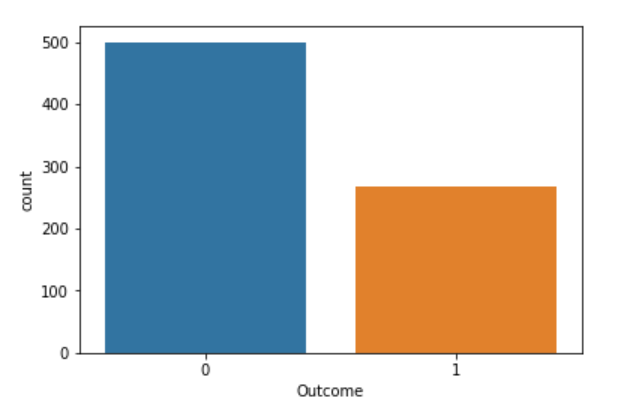
\includegraphics{images/outcome.png}
	\caption{Outcome}
	\label{fig:outcome}
\end{figure}

Całkowita liczba obserwacji wynosi 786.\\

Źródło: https://www.kaggle.com/uciml/pima-indians-diabetes-database


% Please add the following required packages to your document preamble:
\begin{table}[]
	\caption{Opis zbioru danych, cz. 1}
	\label{table:opis}
	\begin{tabular}{@{}llllllllll@{}}
		\toprule
		               & \textbf{Pregnancies} & \textbf{Glucose} & \textbf{BloodPressure} & \textbf{SkinThickness} & \textbf{Insulin} &   &   &   &   \\ \midrule
		\textbf{count} & 768                  & 768              & 768                    & 768                    & 768              &   &   &   &   \\
		\textbf{mean}  & 3.845052             & 120.8945         & 69.10547               & 20.53646               & 79.79948         &   &   &   &   \\
		\textbf{std}   & 3.369578             & 31.97262         & 19.35581               & 15.95222               & 115.244          &   &   &   &   \\
		\textbf{min}   & 0                    & 0                & 0                      & 0                      & 0                &   &   &   &   \\
		\textbf{25\%}  & 1                    & 99               & 62                     & 0                      & 0                &   &   &   &   \\
		\textbf{50\%}  & 3                    & 117              & 72                     & 23                     & 30.5             &   &   &   &   \\
		\textbf{75\%}  & 6                    & 140.25           & 80                     & 32                     & 127.25           &   &   &   &   \\
		\textbf{max}   & 17                   & 199              & 122                    & 99                     & 846              &   &   &   &   \\ \bottomrule
		
	\end{tabular}
\end{table}

% Please add the following required packages to your document preamble:
\begin{table}[]
	\caption{Opis zbioru danych, cz. 2}
	\label{table:opis2}
	\begin{tabular}{@{}llllllllll@{}}
		\toprule
		               & \textbf{BMI} & \textbf{DiabetesPedigreeFunction} & \textbf{Age} & \textbf{Outcome} & \textbf{} &   &   &   &   \\ \midrule
		\textbf{count} & 768          & 768                               & 768          & 768              &           &   &   &   &   \\
		\textbf{mean}  & 31.99258     & 0.471876                          & 33.24089     & 0.348958         &           &   &   &   &   \\
		\textbf{std}   & 7.88416      & 0.331329                          & 11.76023     & 0.476951         &           &   &   &   &   \\
		\textbf{min}   & 0            & 0.078                             & 21           & 0                &           &   &   &   &   \\
		\textbf{25\%}  & 27.3         & 0.24375                           & 24           & 0                &           &   &   &   &   \\
		\textbf{50\%}  & 32           & 0.3725                            & 29           & 0                &           &   &   &   &   \\
		\textbf{75\%}  & 36.6         & 0.62625                           & 41           & 1                &           &   &   &   &   \\
		\textbf{max}   & 67.1         & 2.42                              & 81           & 1                &           &   &   &   &   \\ \bottomrule
	\end{tabular}
\end{table}

\pagebreak
\section{Cel projektu}

Celem projektu jest dokonanie klasyfikacji oraz zbadanie czy u danego pacjenta wystąpi cukrzyca czy nie. Zbadane zostanie także czy dane zawarte w~zbiorze są wystarczające do decyzji o prawdopodobieństwie wystąpienia choroby oraz czy wszystkie z nich wpływają znacząco na wystąpienie choroby.
W projekcie porównane zostaną wyniki skuteczności różnych klasyfikatorów.

\section{Narzędzia}
W celu efetywnej implementacji kolejnych etapów projektu wykorzystano środowisko Jupiter Notebook, a współpracę zespołu umożliwiło repozytorium na serwisie GitHub oraz Overleaf do współdzielenia dokumentacji w \LaTeX.. W projekcie posłużono się językiem Python oraz bibliotekami poświęconymi analizie danych i uczeniu maszynowemu, takimi jak: NumPy, Pandas, SciKit-learn. Do wytworzenia wykresów zastosowano biblioteki Matplotlib oraz Seaborn. 

\section{Analiza zbioru}

Zanim przystąpimy do próby klasyfikacji, dane zostały odpowiednio przygotowane. Sprawdzone zostają wiersze, w których występują zera oraz wartości odstające.

\subsection{Wartości zerowe}

\begin{figure}
	\begin{adjustwidth}{-3.3cm}{}
		\centering
		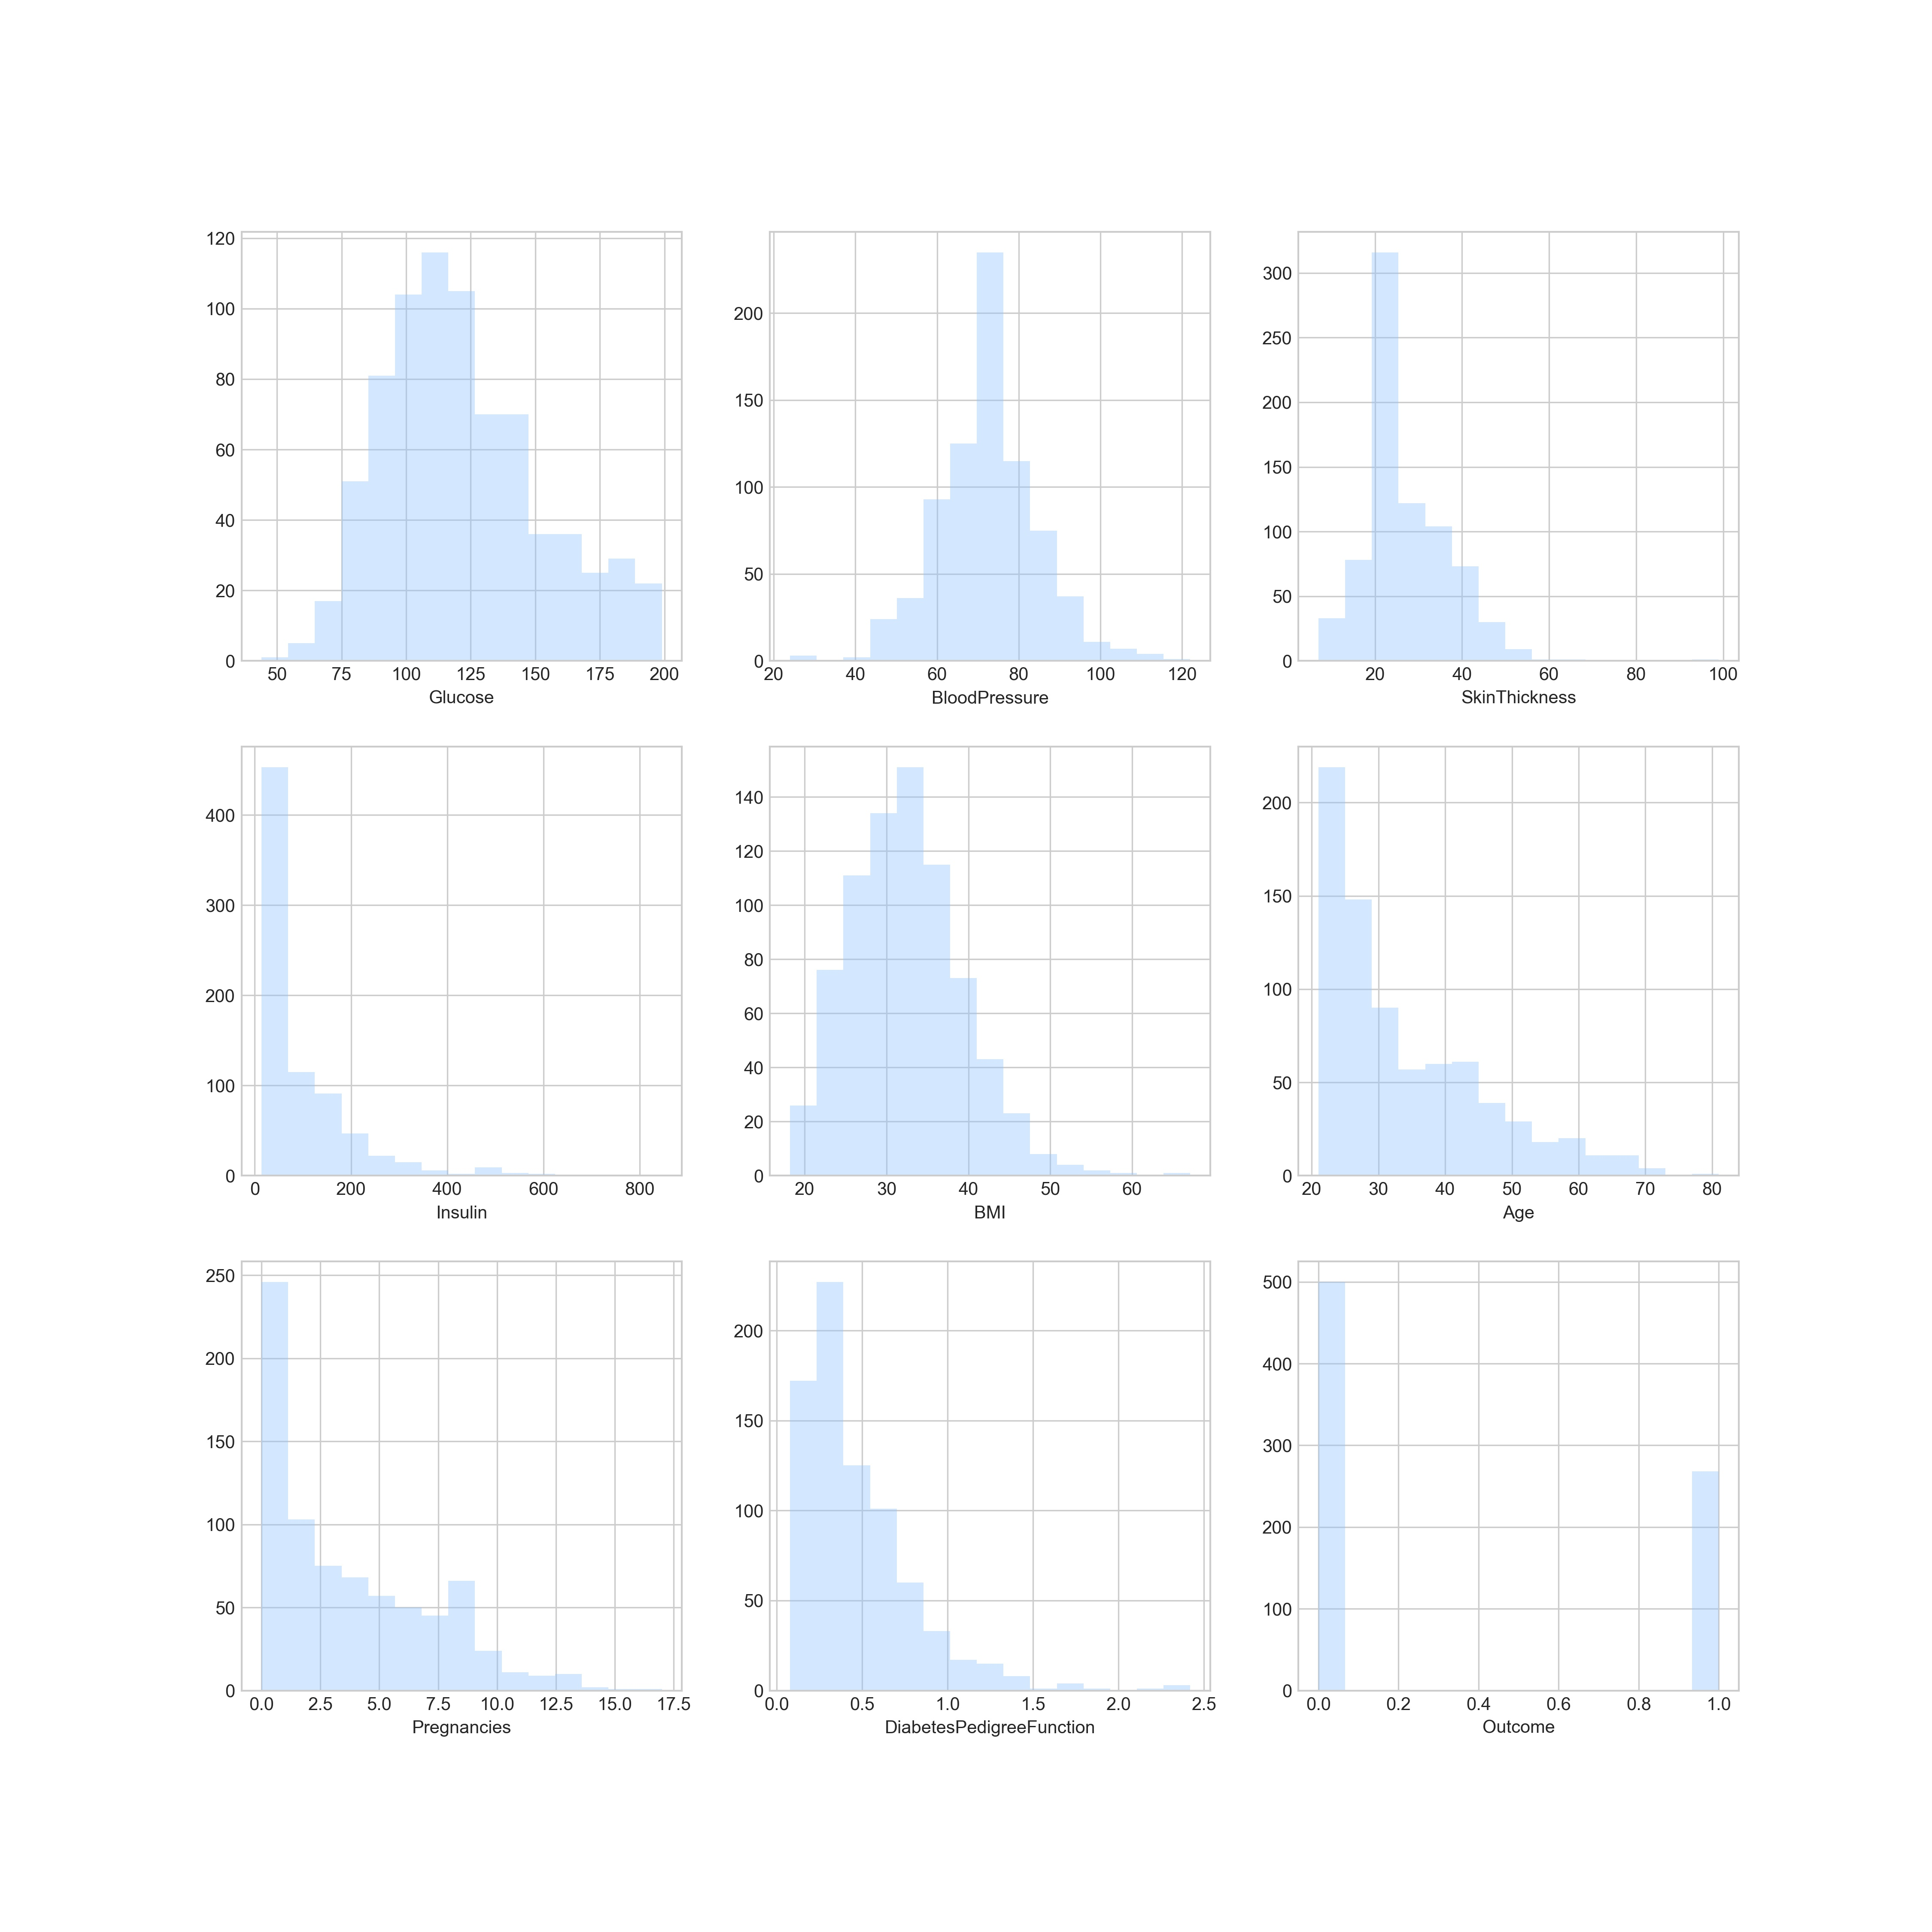
\includegraphics[width=1.5\textwidth]{images/histograms_median.jpg}
		\caption{Histogramy po zastąpieniu wartości 0 medianą}
		\label{fig:outliers}
	\end{adjustwidth}
\end{figure}

\begin{figure}
	\begin{adjustwidth}{-3.3cm}{}
		\centering
		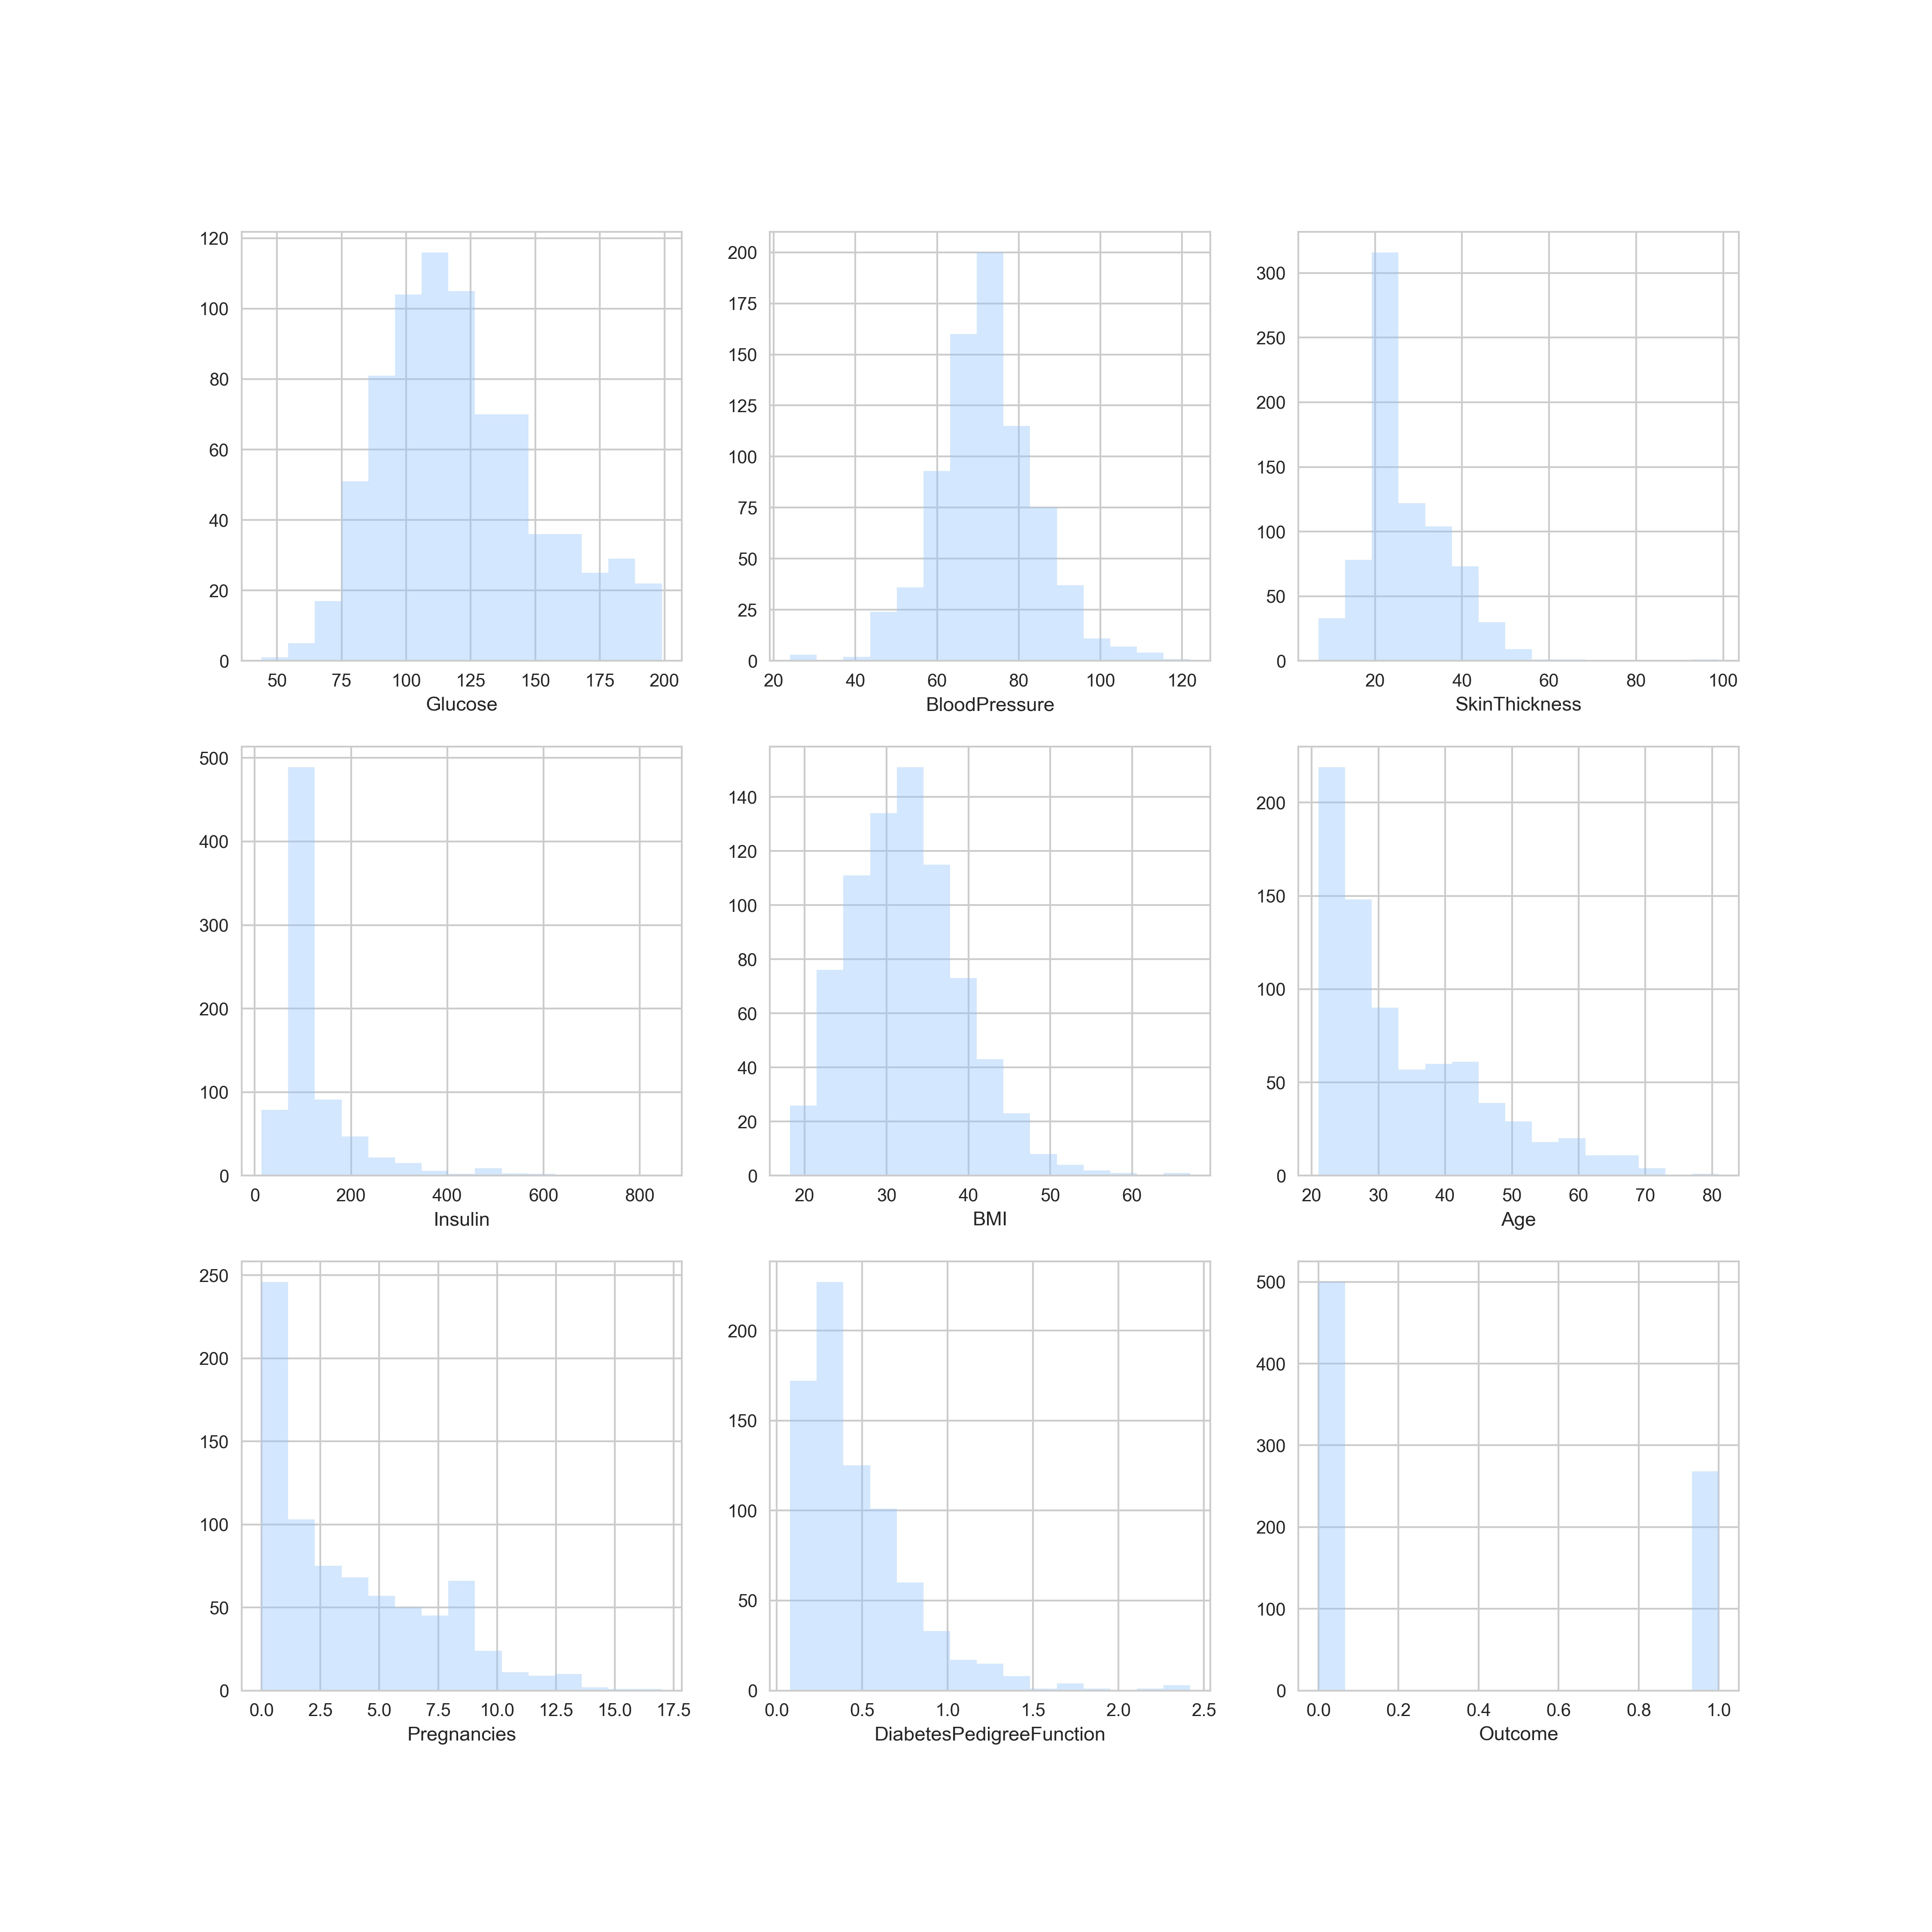
\includegraphics[width=1.5\textwidth]{images/histograms_average.jpg}
		\caption{Histogramy po zastąpieniu wartości 0 średnią}
		\label{fig:outliers}
	\end{adjustwidth}
\end{figure}

Z tabel \ref{table:opis} oraz \ref{table:opis2} wynika, że istnieją wartości zerowe w kolumnach \textit{Pregnancies, Glucose, BoloodPressuure, SkinThickness, Insulin, BMI}. Z medycznego punktu widzenia, cechy w badanym zbiorze nie mogą być równe zeru, świadczy to o braku poprawności danych danych. W~przypadku pierwszej kolumny wartości zerowe są poprawne - jest to informacja, że dana kobieta nie była w~ciąży. W przypadku reszty obserwacji dane zostają zamienione na \textbf{średnią wartość} w kolumnie, \textbf{medianę} oraz zostają całkowicie \textbf{usunięte}. Wszystkie trzy przypadki posłużą jako dane testowe.

\subsection{Wartości odstające}

\begin{figure}
	\begin{adjustwidth}{-3.3cm}{}
		\centering
		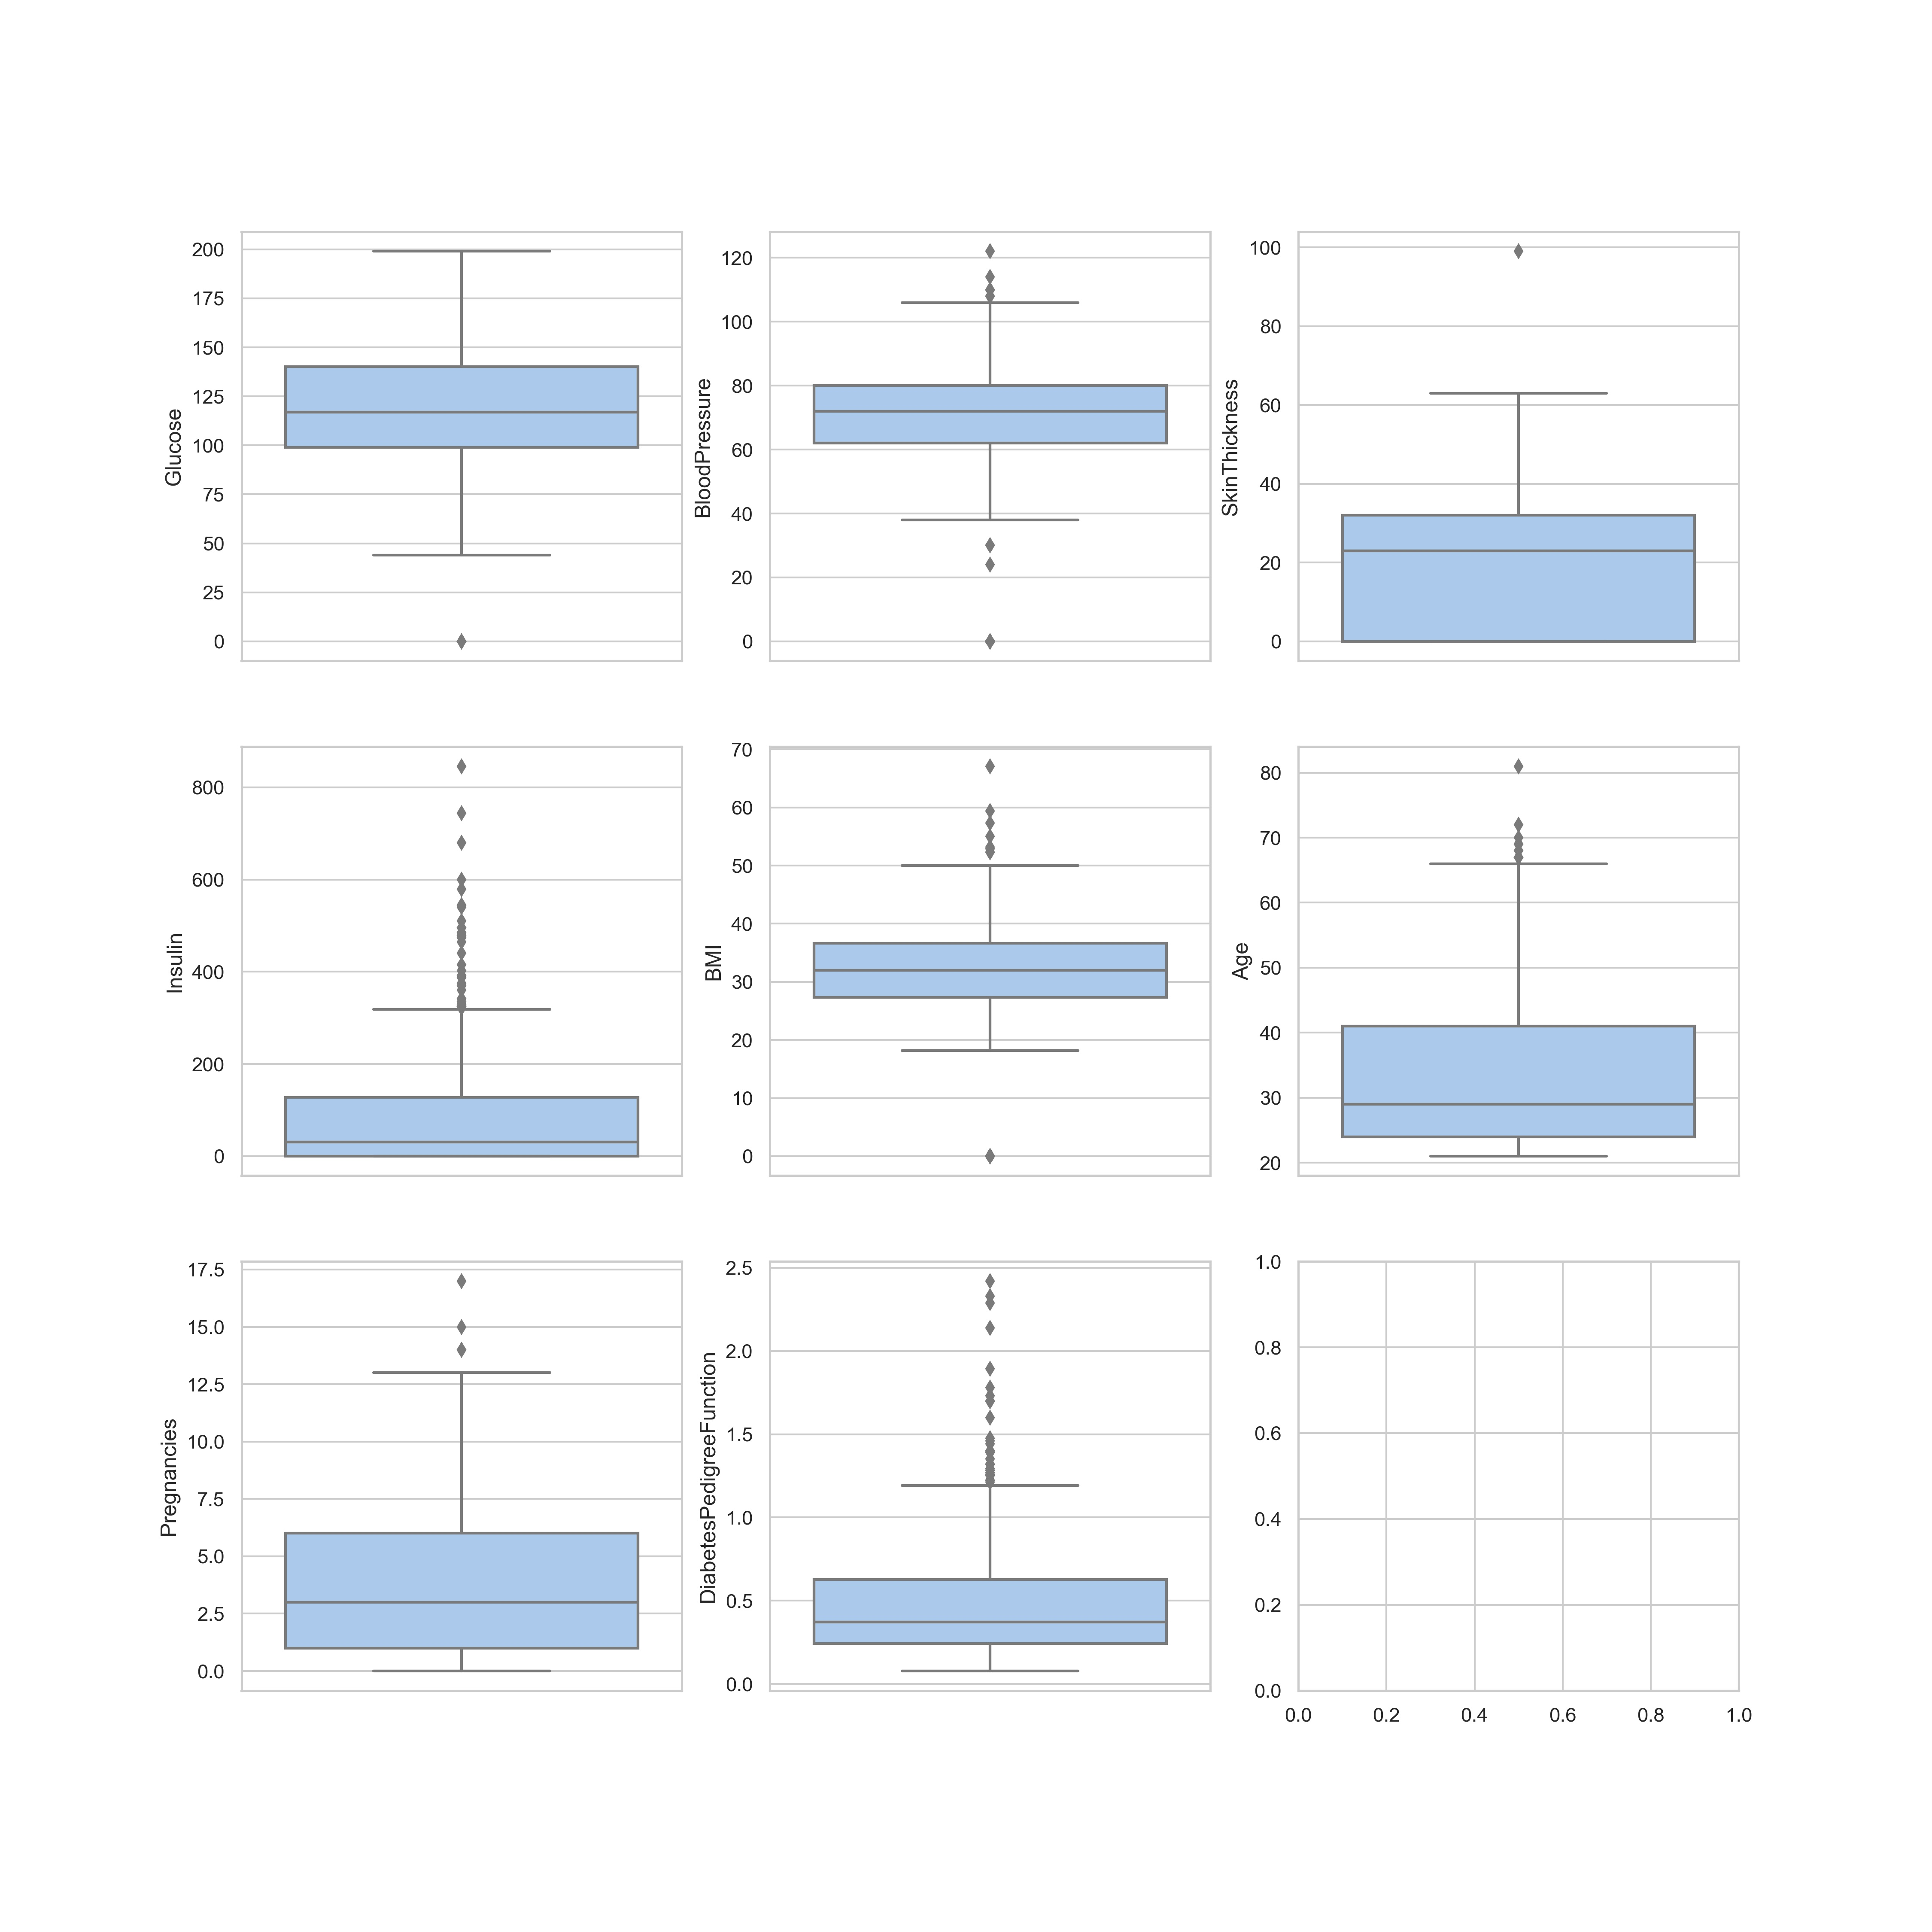
\includegraphics[width=1.5\textwidth]{images/boxplots.jpg}
		\caption{Wartości odstające}
		\label{fig:outliers}
	\end{adjustwidth}
\end{figure}

Pomimo, że w zbiorze dla niektórch cech występują wartości odstające nie zostały one usunięte. Dla niektórych zmiennych z powodów medycznych nie został zdefiniowany górny lub dolny zakres mierzalny. W niektórych przypadkach wartości odstające mogą również świadczyć o objawach choroby, a więc usunięcie ich ze zbioru wpłynęłoby niekorzystnie na dopasowanie modelu.

\subsection{Selekcja cech}


Przy użyciu \textit{ExtraTreesClassifier} z modelu zostały usunięte cechy, które nie zostały uznane za istotne. Dzięki tej redukcji, trening modelu może być przeprowadzony w krótszym czasie bez straty na jakości. Cechy z najniższym wynikiem zostają odrzucone. Wyniki istotności wg. \textit{ExtraTreesClassifier} zostały przedstawione w tabeli \ref{table:selekcja}.
	
\begin{table}[H]
	\caption{Wyniki przeprowadzenia eksperymentu selekcji cech}
	\label{table:selekcja}
	\begin{adjustwidth}{-3cm}{}
		\begin{tabular}{@{}lllllllll@{}}
			\toprule
			  & Pregnancies                  & Glucose                      & BloodPressure                                        & SkinThickness                & Insulin                                              & BMI                         & DiabetesPdigFun               & Age                          \\ \midrule
			  & \multicolumn{1}{c}{0.108638} & \multicolumn{1}{c}{0.245338} & \multicolumn{1}{c}{\cellcolor[HTML]{FE0000}0.083665} & \multicolumn{1}{c}{0.084513} & \multicolumn{1}{c}{\cellcolor[HTML]{FE0000}0.081918} & \multicolumn{1}{c}{0.15441} & \multicolumn{1}{c}{0.1096581} & \multicolumn{1}{c}{0.127862} \\ \bottomrule
		\end{tabular}
	\end{adjustwidth}
\end{table}	
	
Zgodnie z powyższą tabelą postanowiono odrzucić cechy: BloodPressure oraz Insullin.
	
\subsection{Normalizacja}
Normalizacja jest jednym z najważniejszych przekształceń dokonywanych na danych. W przypadku kiedy zakresy wartości różnych cech znacznie się różnią, klasyfikator może usnać wyższe wartości za bardziej wpływające na model \cite{geron}.
Do normalizacji użyto:
\begin{itemize}
	\item \textit{MinMaxScaler}
	      \begin{equation}
	      	x' = \frac{x - min(x)}{max(x) - min(x)}
	      \end{equation}
	\item {StandardScaler}
	      \begin{equation}
	      	x' = \frac{x - \overline{x}}{\sigma}
	      \end{equation}
\end{itemize}
Najlepsze wyniki zostały uzyskane w przypadku \textit{StandardScaler}.

\section{Walidacja krzyżowa}
Przed przystąpieniem do klasyfikacji zastosowano podział zbioru danych na dane treningowe oraz testowe, a następnie wykorzystano 5-krotną walidację krzyżową. Proces ten stosuje się w celu minimalizacji problemu nadmiernego dopasowania (\textit{overfitting}). Dzięki niemu można uzyskać informacje takie jak dokładność modelu (\textit{accuracy}) czy macierz pomyłek, które umożliwiają ocenę jakości modelu.
	

\section{Wyniki}
Do klasyfikacji zostało użytych siedem różnych klasyfikatorów w celu porównania wyników. Dla każdego klasyfikatora zastosowano metodę \textit{GridSearch}, w celu znalezienia najlepszych parametrów modelu. Zostały wykonanane łacznie $334$ porównania dla  5-krotnej walidacji krzyżowej. Dzięki wyspecyfikowaniu parametru \textit{n\_jobs} obliczenia wykonywane były szybciej przy użyciu kilku rdzeni procesora. Poniżej przedstawiono parametry modeli, którymi posłużono się w dalszej części badań.
\begin{itemize}
	\item{Maszyna wektorów nośnych (SVM)}
	\begin{itemize}
		\item{C = 1 (parametr kary)}
		\item{gamma = 0.01 (współczynnik jądra)}
		\item{kernel = rbf (typ jądra)}
	\end{itemize}
	    
	\begin{figure}[h!]
		\centering
		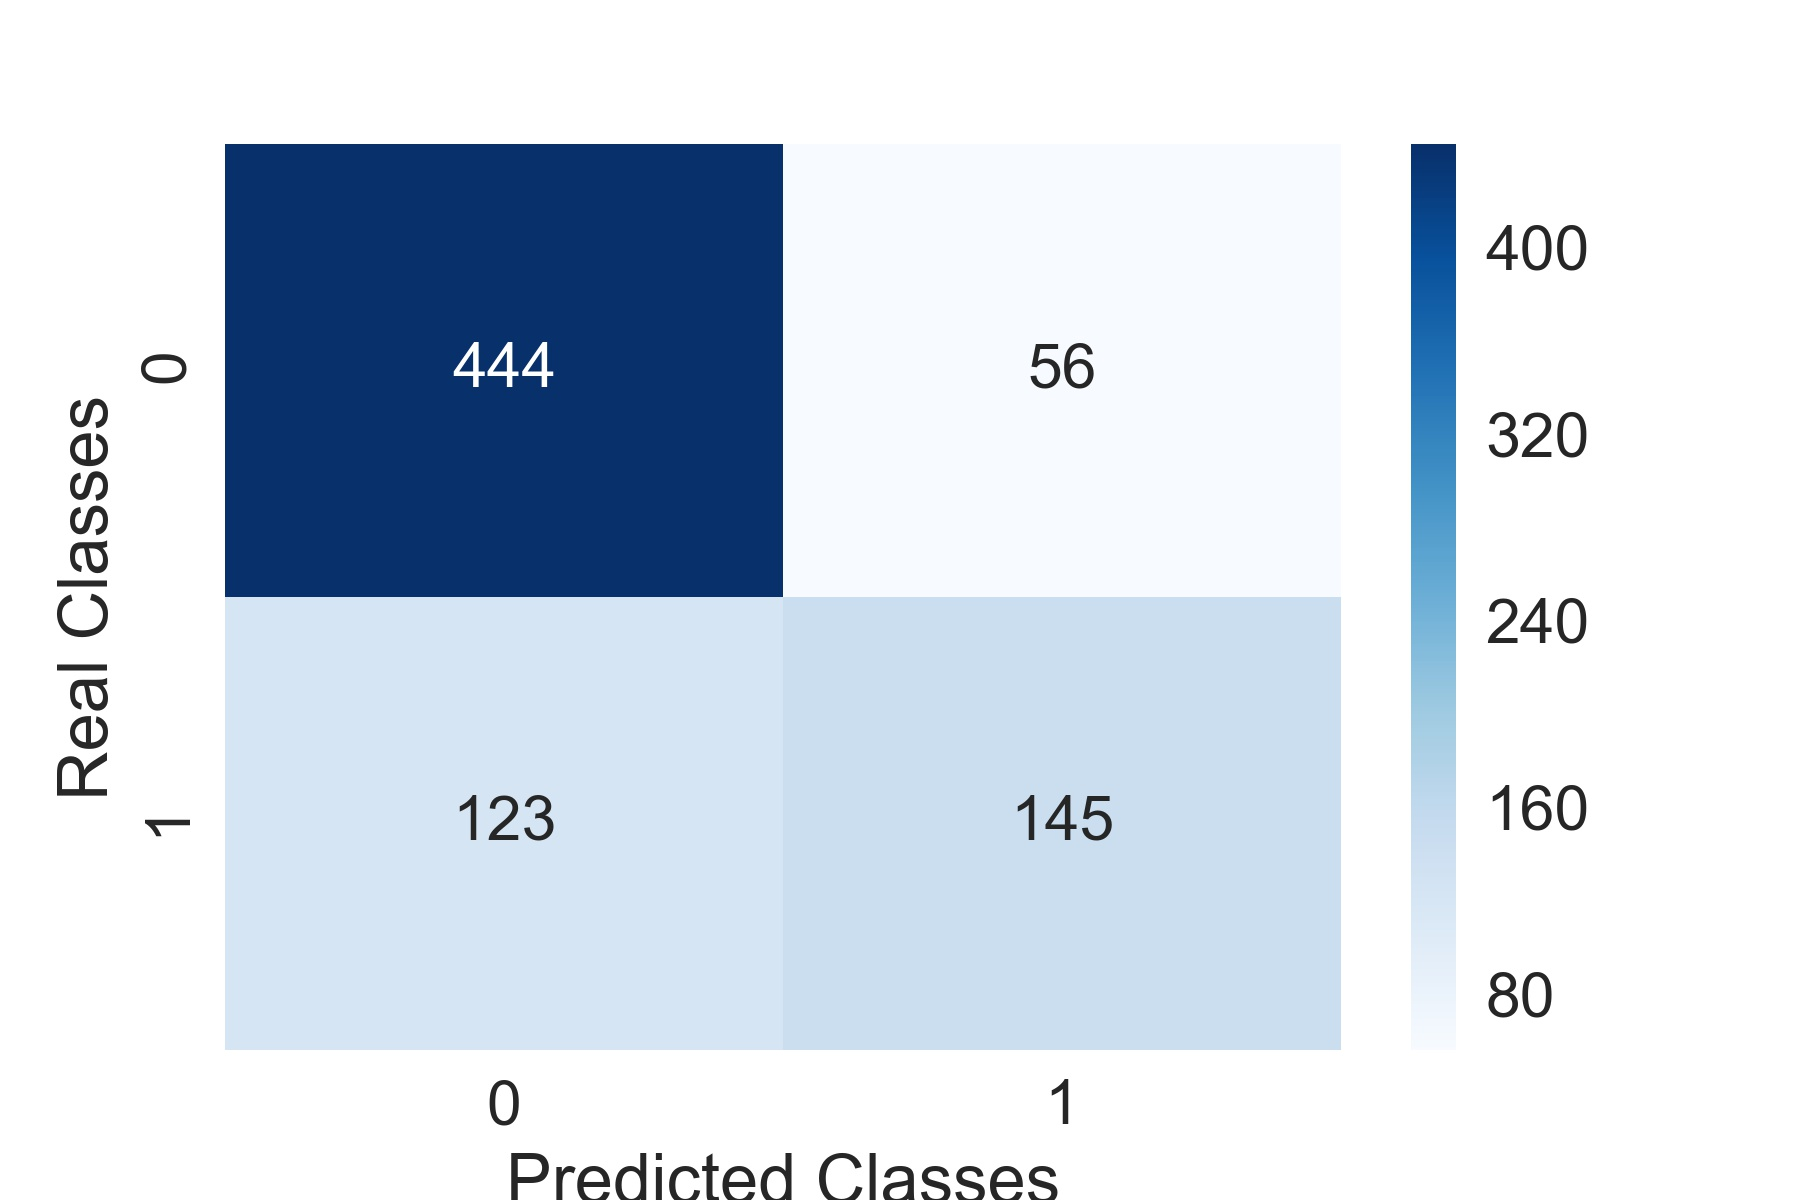
\includegraphics[width=0.7\textwidth]{images/confusion_svc.jpg}
		\caption{Macierz pomyłek dla klasyfikatora SVC}
		\label{fig:outliers}
	\end{figure}
	
	\item{K najbliższych sąsiadów (KNN)}
	\begin{itemize}
		\item{n\_neighbors = 3 (liczba sąsiadów)}
		\item{weights = uniform (funkcja wagowa)}
	\end{itemize}
	    
	\begin{figure}[H]
		\centering
		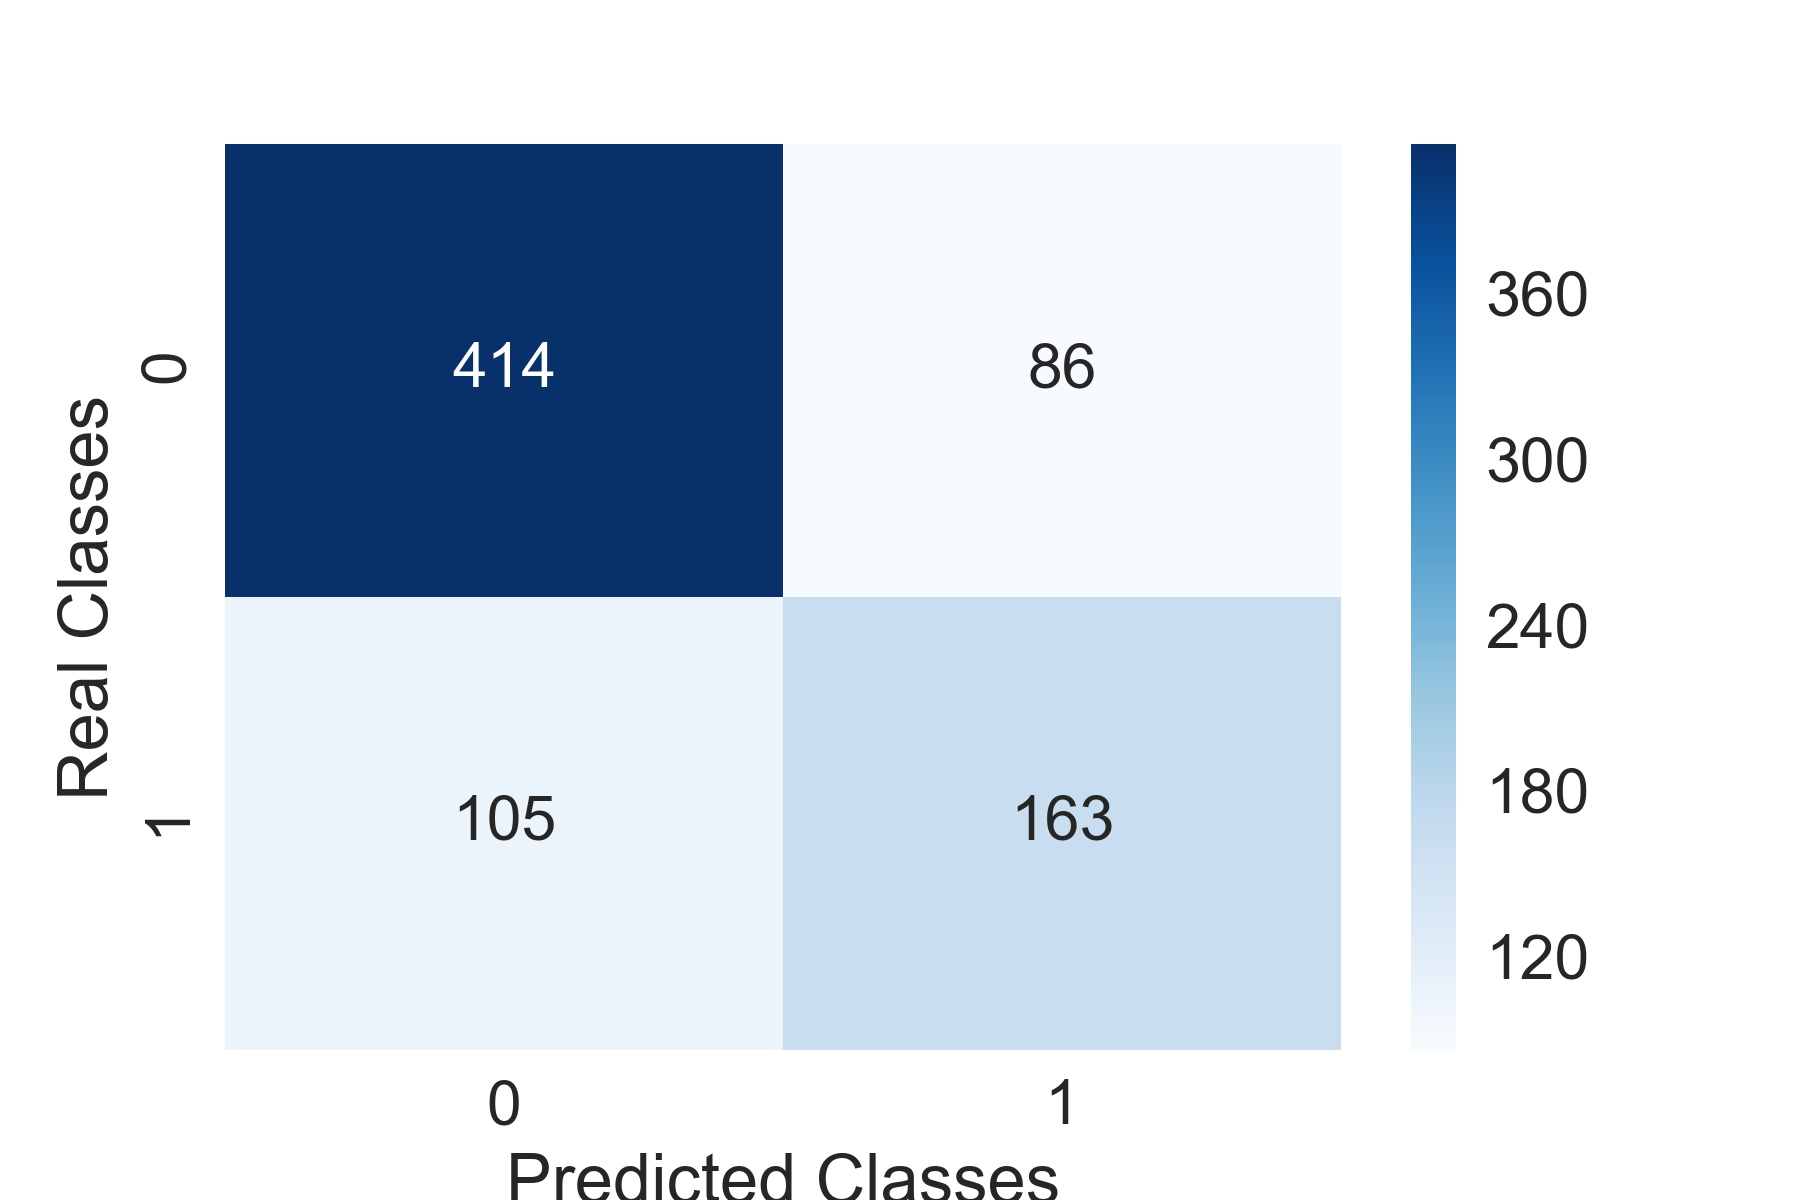
\includegraphics[width=0.7\textwidth]{images/confusion_knn.jpg}
		\caption{Macierz pomyłek dla klasyfikatora KNN}
		\label{fig:outliers}
	\end{figure}
	\item{Drzewo decyzyjne}
	\begin{itemize}
		\item{max\_depth = 6 (maksymalna głębokość drzewa)}
	\end{itemize}
	\begin{figure}[H]
		\centering
		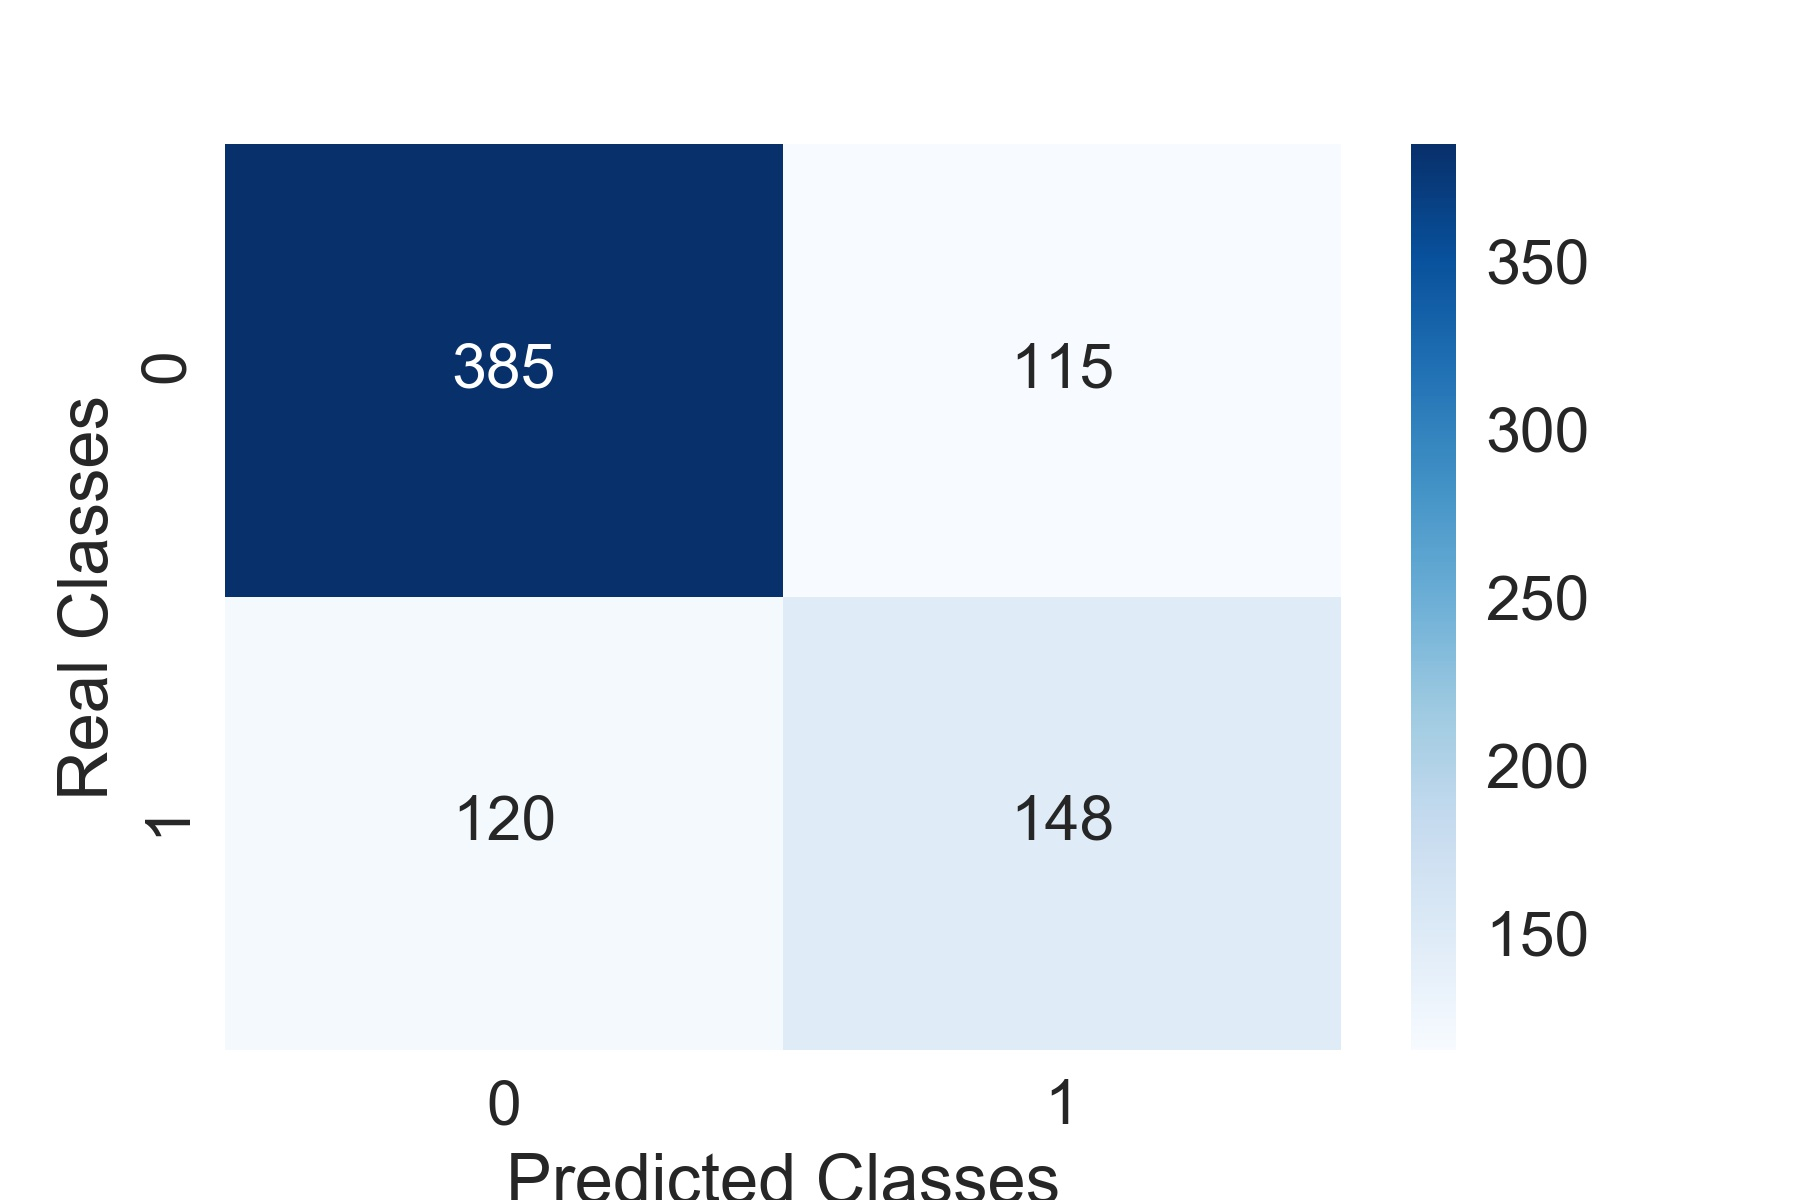
\includegraphics[width=0.7\textwidth]{images/confusion_dtree.jpg}
		\caption{Macierz pomyłek dla klasyfikatora Decision Tree}
		\label{fig:outliers}
	\end{figure}
	% https://scikit-learn.org/stable/modules/generated/sklearn.ensemble.RandomForestClassifier.html
	\item{Las losowy}
	\begin{itemize}
		\item{max\_depth =  3 (maksymalna głębokość drzewa)}
		\item{max\_features = 4 (liczba zmiennych rozpatrywanych przy budowie drzewa)}
		\item{min\_samples\_split = 3 (minimalna liczba próbek potrzebna to rozgałęzienia)}
		\item{bootstrap = True (czy wykorzystywane są próbki typu bootstrap )}
		\item{criterion =  gini (funkcja mierząca jakość rozgalęzienia)}
		\item{n\_estimators = 10 (liczba drzew w lesie)}
	\end{itemize}
	    
	\begin{figure}[H]
		\centering
		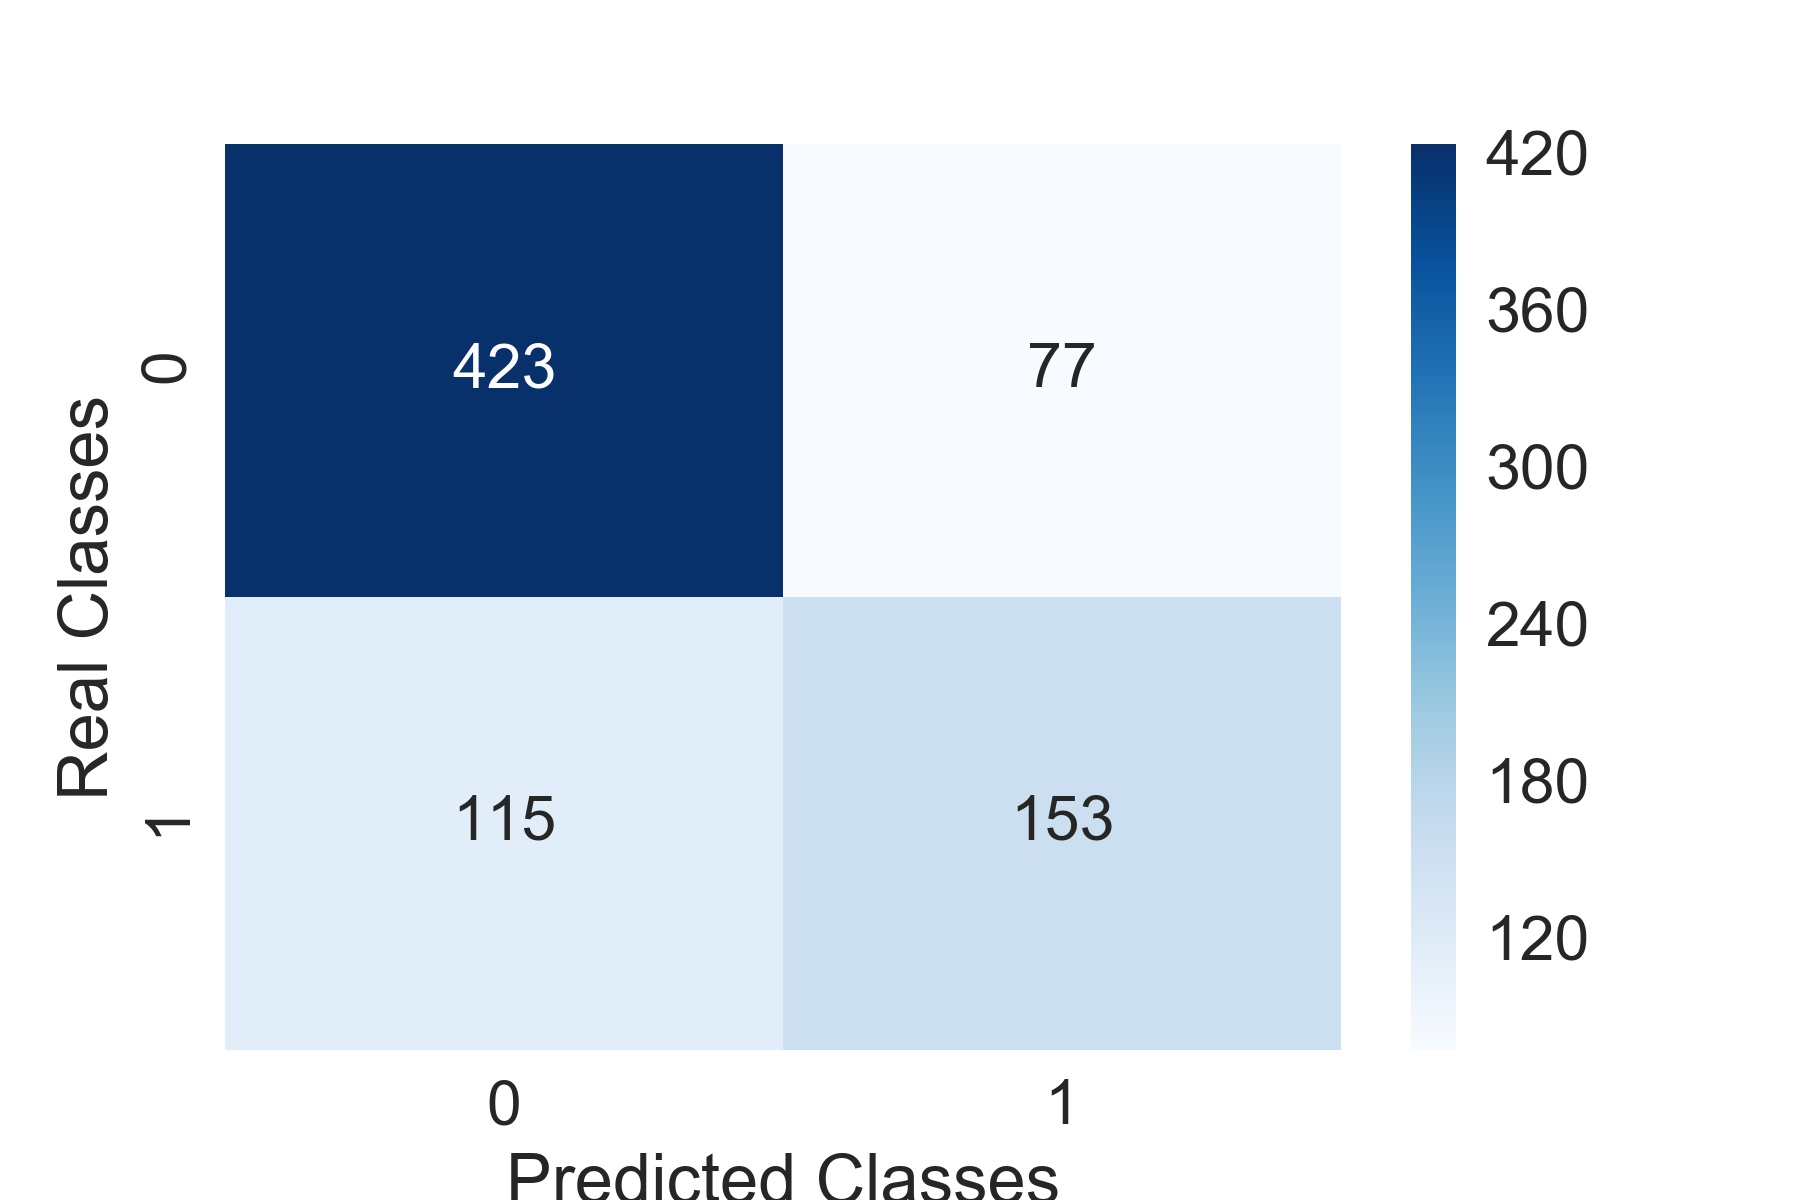
\includegraphics[width=0.7\textwidth]{images/confusion_rfc.jpg}
		\caption{Macierz pomyłek dla klasyfikatora Las Losowy}
		\label{fig:outliers}
	\end{figure}
	
	\item{Regresja logistyczna}
	\begin{itemize}
		\item{C = 0.1 (paramter kary)} %??? dok: "Inverse of regularization strength"
		\item{penalty = l1 (norma wykorzystywana w procesie karania)}
	\end{itemize}
	    
	\begin{figure}[H]
		\centering
		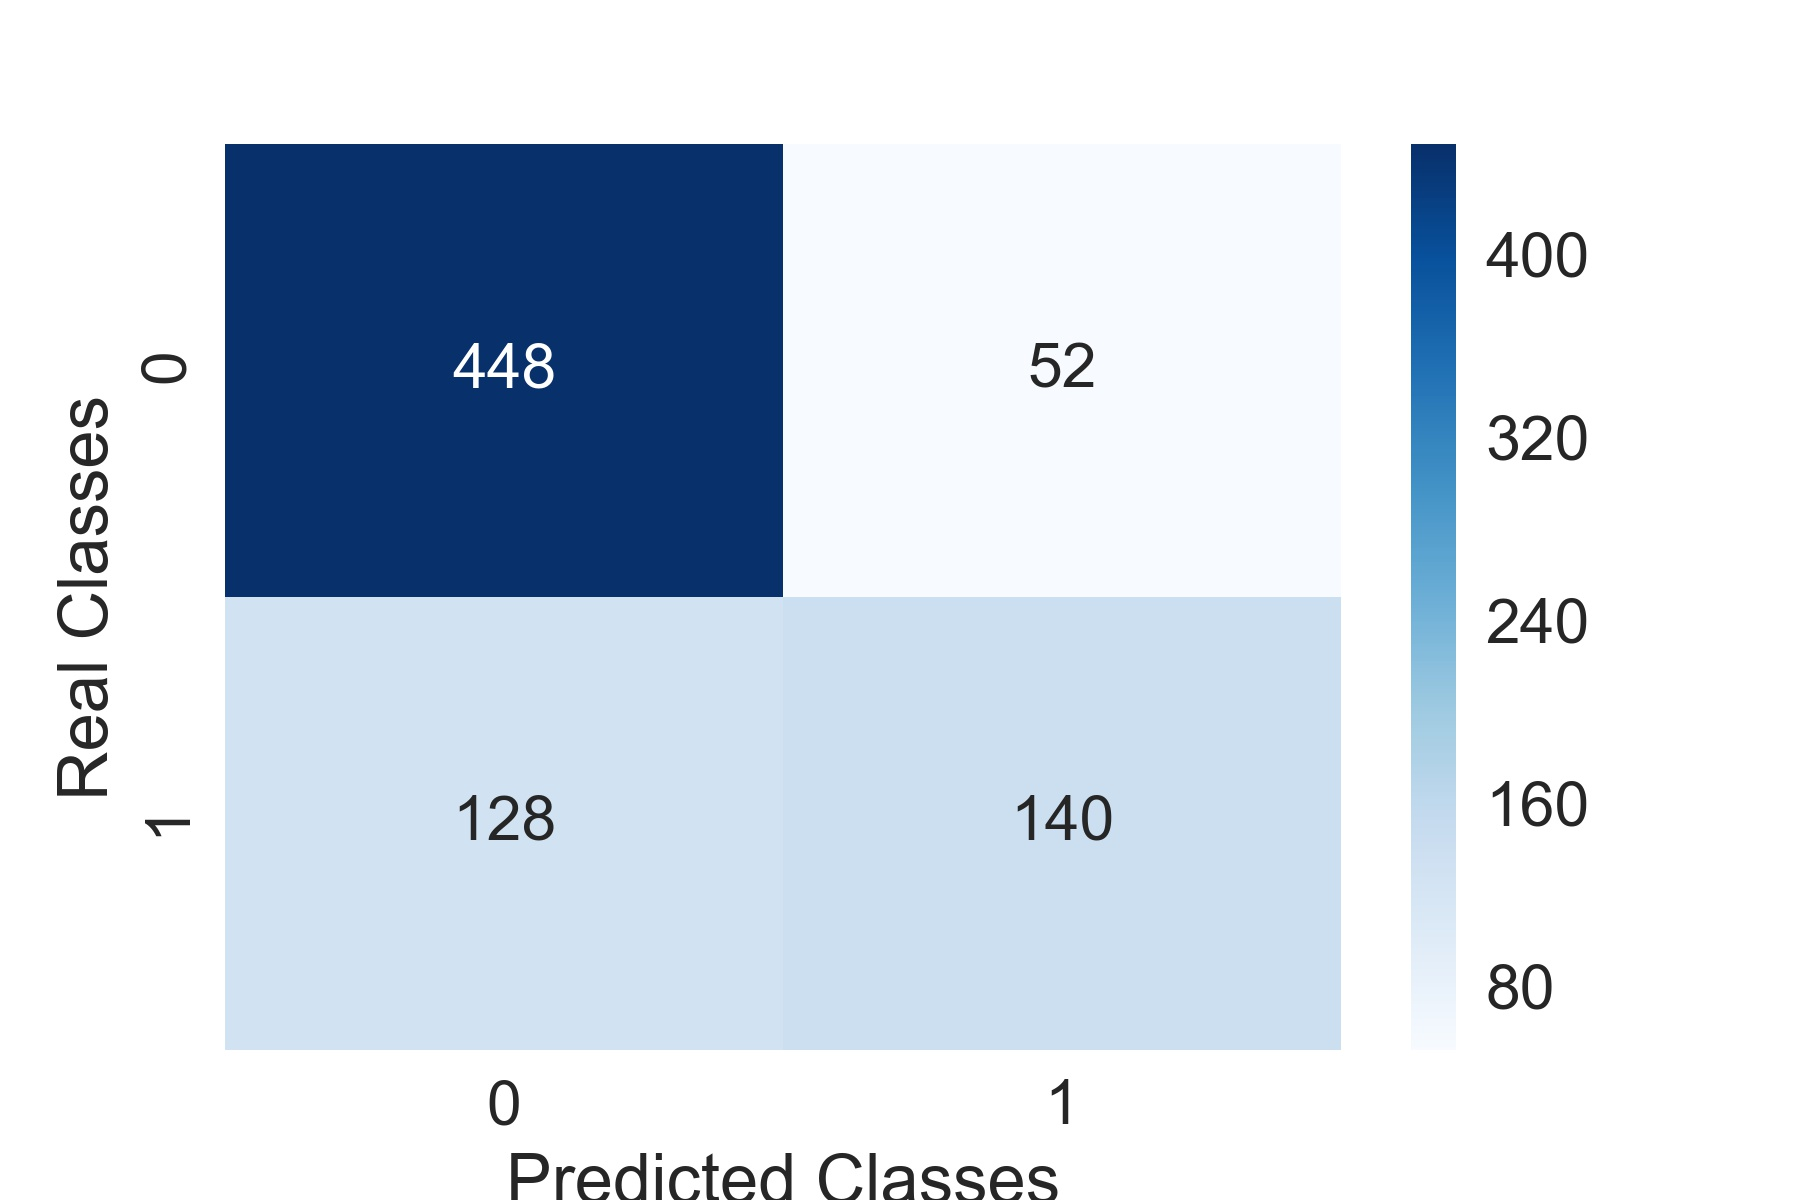
\includegraphics[width=0.7\textwidth]{images/confusion_log.jpg}
		\caption{Macierz pomyłek dla klasyfikatora Regresji Logistycznej}
		\label{fig:outliers}
	\end{figure}
	\item{Naiwny klasyfikator bayesowski}
	
	\begin{figure}[H]
		\centering
		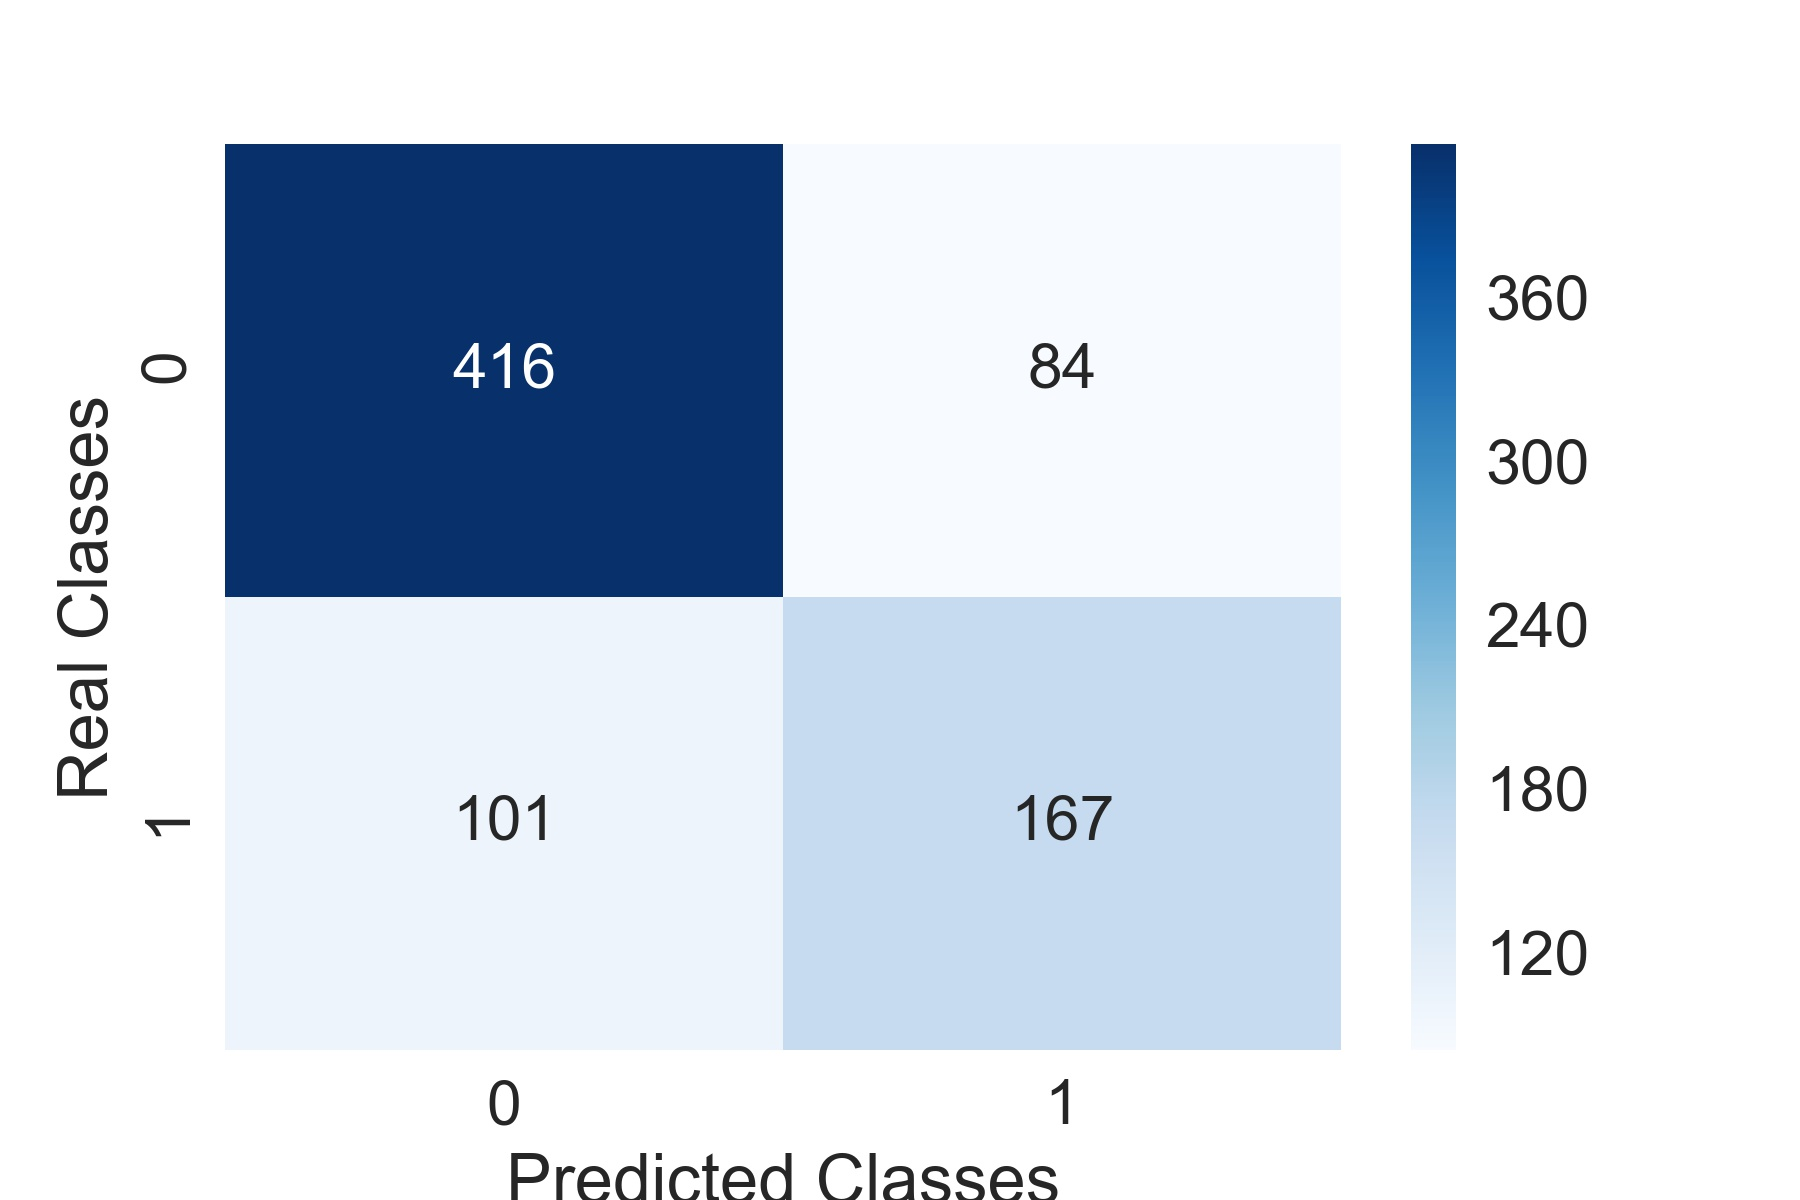
\includegraphics[width=0.7\textwidth]{images/confusion_gnb.jpg}
		\caption{Macierz pomyłek dla Naiwny klasyfikatora bayesowskiego}
		\label{fig:outliers}
	\end{figure}
	
	\item{Ada Boost}
	\begin{figure}[H]
		\centering
		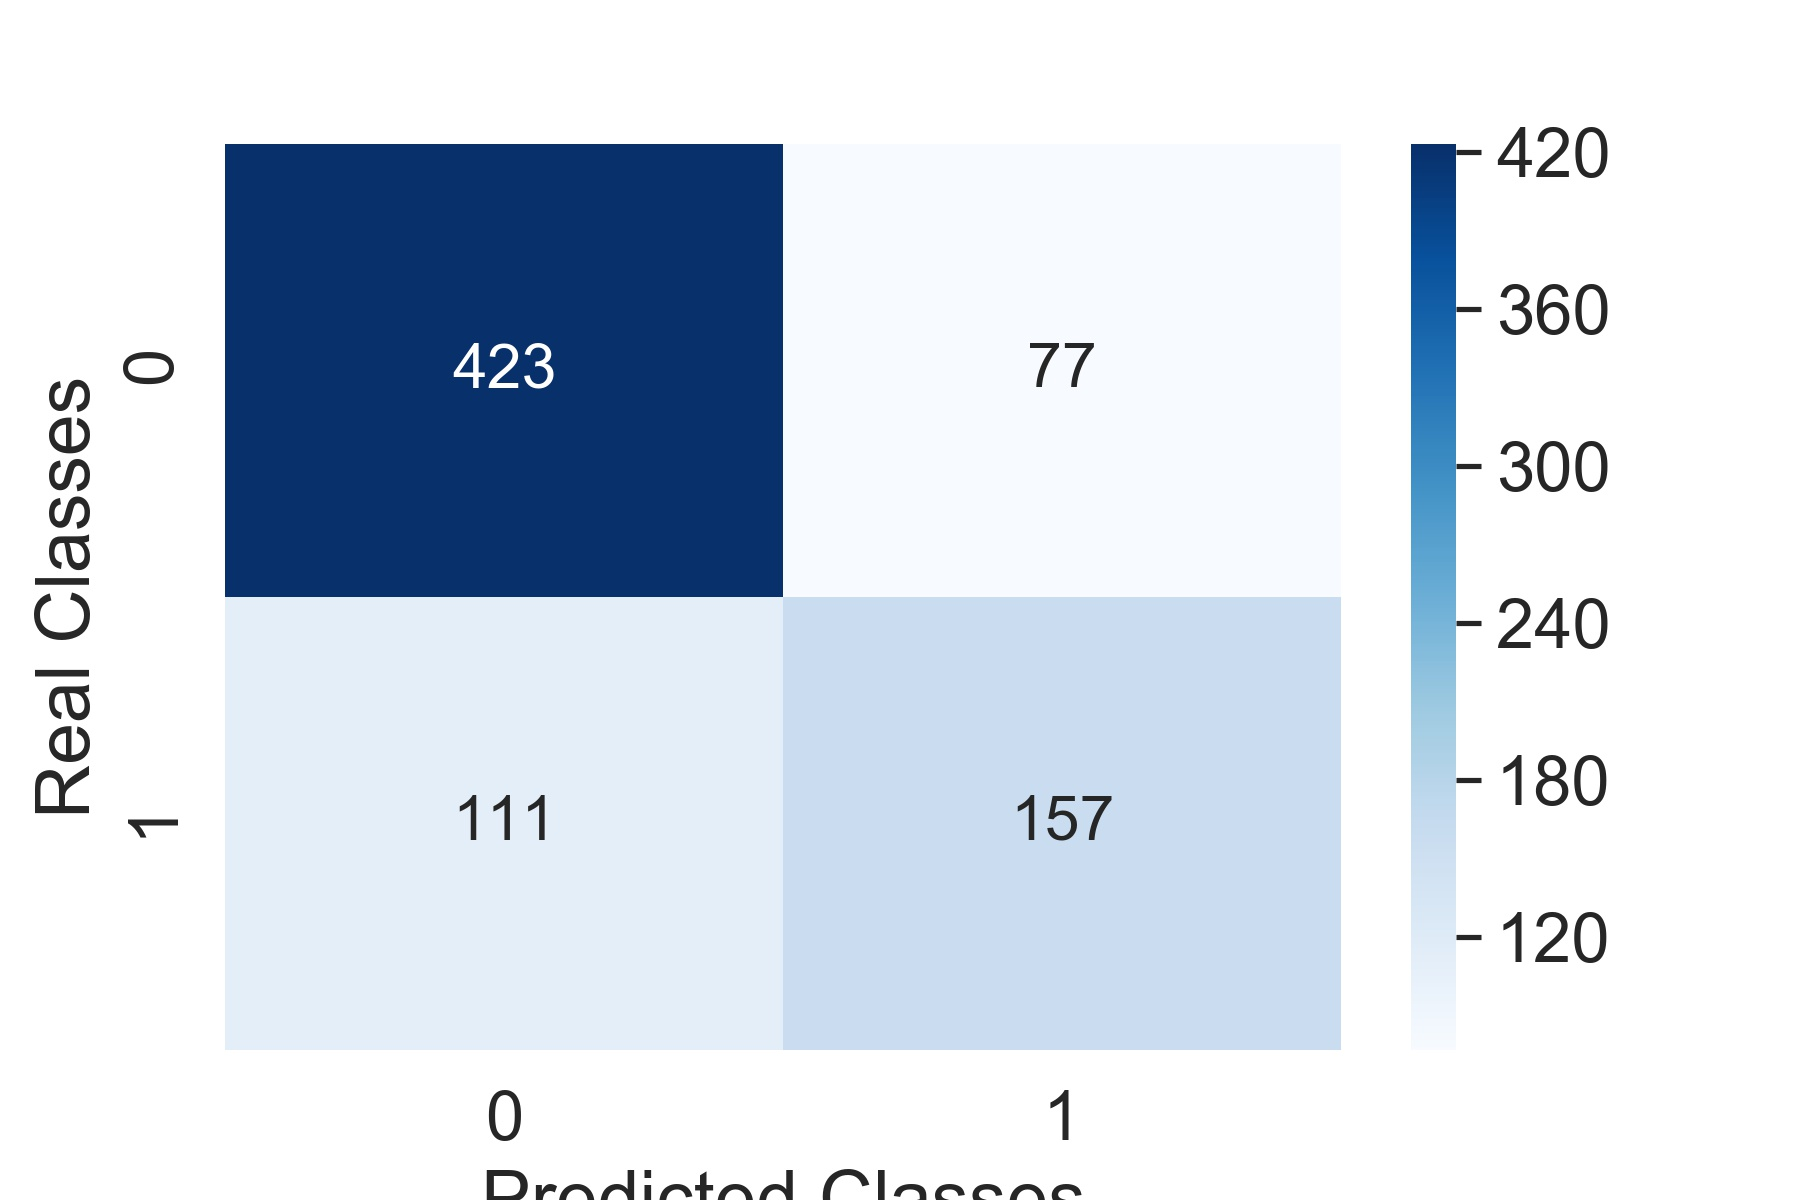
\includegraphics[width=0.7\textwidth]{images/confusion_adb.jpg}
		\caption{Macierz pomyłek dla klasyfikatora Ada Boost}
		\label{fig:outliers}
	\end{figure}
	
\end{itemize}
%Tabela wynikow

\begin{table}[]
	\caption{Ostateczne wyniki dokladności klasyfikatorów dla najlepiej dopasowanych parametrów}
	\begin{tabular}{@{\hspace{-2cm}}lccccccc}
		\hline
		                     & \multicolumn{1}{l}{\textbf{SVC}} & \multicolumn{1}{l}{\textbf{KNN}} & \multicolumn{1}{l}{\textbf{Dec. Tree}} & \multicolumn{1}{l}{\textbf{Rnd Forest}} & \multicolumn{1}{l}{\textbf{Log Reg}}                  & \multicolumn{1}{l}{\textbf{Gaussian naive}} & \multicolumn{1}{l}{\textbf{Ada Boost}} \\ \hline
		\textbf{Std Scaller} & \cellcolor[HTML]{FFC702}0.7922   & \cellcolor[HTML]{FD6864}0.7619   & \cellcolor[HTML]{FD6864}0.7706         & \cellcolor[HTML]{FD6864}0.7706          & \cellcolor[HTML]{009901}{\color[HTML]{000000} 0.8052} & \cellcolor[HTML]{FFC702}0.78                & \cellcolor[HTML]{FFC702}0.7965         \\
		\textbf{Min-Max}     & \cellcolor[HTML]{FFC702}0.7965   & \cellcolor[HTML]{FE0000}0.7449   & \cellcolor[HTML]{FD6864}0.7619         & \cellcolor[HTML]{FD6864}0.7749          & \cellcolor[HTML]{FFC702}0.7965                        & \cellcolor[HTML]{FFC702}0.78                & \cellcolor[HTML]{FFC702}0.7965         \\
		\textbf{Brak}        & \cellcolor[HTML]{FFC702}0.7965   & \cellcolor[HTML]{FE0000}0.7449   & \cellcolor[HTML]{FE0000}0.7446         & \cellcolor[HTML]{FFC702}0.7965          & \cellcolor[HTML]{FFC702}0.7965                        & \cellcolor[HTML]{FFC702}0.78                & \cellcolor[HTML]{FFC702}0.7965         
	\end{tabular}
\end{table}

%koniec tabeli wynikow
\begin{figure}[H]
	\centering
	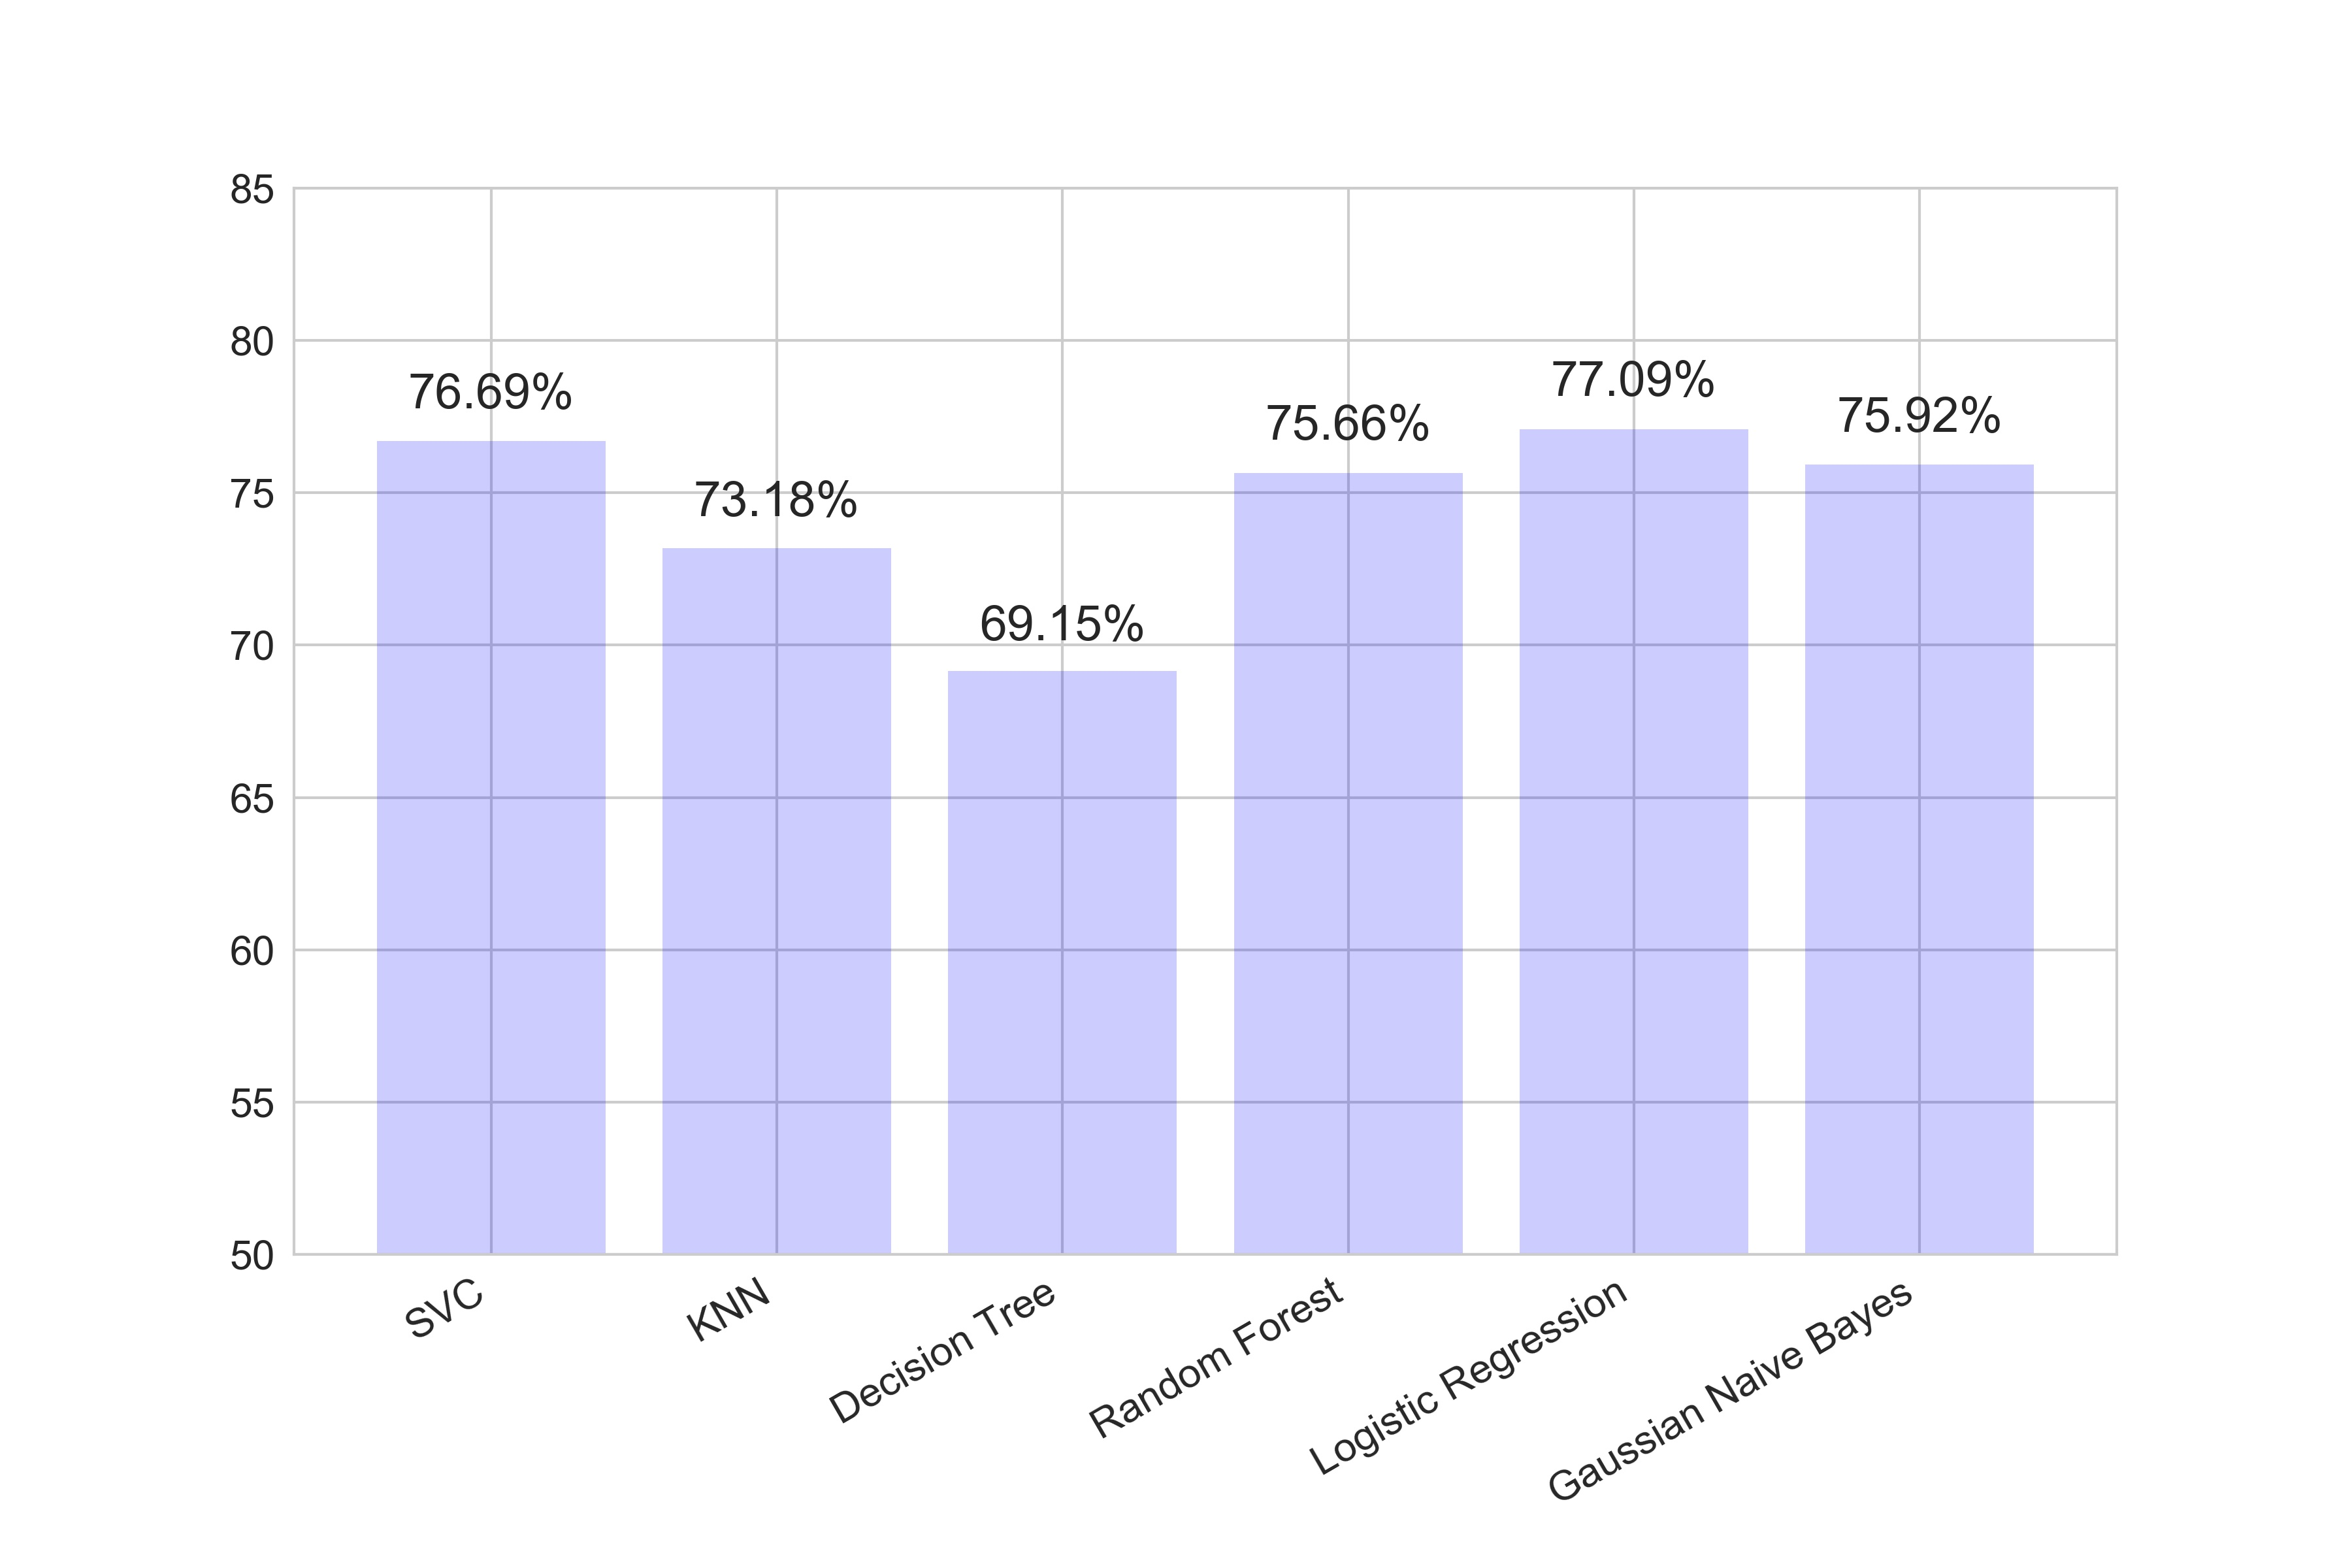
\includegraphics[width=1.2\textwidth]{images/classificators_accuracy.jpg}
	\caption{Dokładność klasyfikatorów}
	\label{fig:accuracy}
\end{figure}

\section{Wnioski}
Zdecydowanie najbardziej pracochłonną częścią projektu była sama analiza i przygotowanie danych wykorzystanych w późniejszej klasyfikacji. Jest też to najistotniejszy element tego typu projektów. Niepoprawne próbki, czyli te które zawierały wartości zerowe w niektórych kolumnach stanowiły większość zbioru i bez zastosowania odpowiednich metod wynik klasyfikacji byłby dużo słabszy. Kolejnym wnioskiem, który nasuwa się po zakończeniu prac jest to, że wynik rzędu 80\% skuteczności klasyfikatora dla zastosowań medycznych nie jest wynikiem zadowalającym. W rzeczywistym przypadku nie można pozwolić sobie na tak duży błąd. Być może udało by się usyzkać lepszy efekt posiadająć wyniki większej ilości badań, bądź dane uzupełnione o brakujące wartości.



\newpage
\begin{thebibliography}{9}
	
	\bibitem{sugarLevel}
	https://www.diabetes.co.uk/diabetescare/blood-sugar-level-ranges.html
	\bibitem{pressure}
	http://www.bloodpressureuk.org/BloodPressureandyou/Thebasics/Bloodpressurechart)
	\bibitem{bmi}
	https://pl.wikipedia.org/wiki/Wskaźnikmasyciała
	\bibitem{overfitting}
	https://en.wikipedia.org/wiki/Cross-validation\_(statistics)
	\bibitem{gridsearch}   
	https://en.wikipedia.org/wiki/Hyperparameter\_optimization\#Grid\_search
	    
	\bibitem{geron}   
	Aurélien Géron, ,,Uczenie maszynowe z użyciem Scikit-Learn i TensorFlow.''
	    
\end{thebibliography}


\end{document}